%-------------------- begin preamble ----------------------

\documentclass
[twocolumn,
secnumarabic,
nobibnotes,
aps,
prl,
reprint,
groupedaddress,
amsmath,
amssymb,
]{revtex4-2}
\usepackage[caption=false]{subfig}
\usepackage{relsize,makeidx,color,setspace,amsfonts}
\usepackage{mathtools}


\usepackage{listings}
\lstset{
    language=Python,
    inputencoding=utf8,
    extendedchars=true,
    literate={ø}{{\o}}1 {å}{{\r a}}1 {Å}{{\r A}}1 {æ}{{\ae}}1,
    backgroundcolor=\color{white},
    basicstyle=\footnotesize\ttfamily,
    breakatwhitespace=false,
    breaklines=true,
    captionpos=b,
    commentstyle=\itshape\color{purple!60!black},
    frame=single,
    %identifierstyle=\color{orange},
    keepspaces=true,
    keywordstyle=\bfseries\color{violet},
    numbers=left,
    numbersep=5pt,
    numberstyle=\tiny\color{black},
    rulecolor=\color{black},
    showstringspaces=false,
    showtabs=false,
    stepnumber=1,
    stringstyle=\color{purple!60!black},
    tabsize=2,
    title=\lstname
  }
\usepackage{dcolumn}% Align table columns on decimal point
\usepackage[table]{xcolor}
\usepackage{bm,ltablex,microtype}
\usepackage{longtable}
\usepackage{siunitx}
\usepackage{algorithm2e}
\usepackage{csvsimple}
\usepackage{url}
\renewcommand{\UrlFont}{\small\tt}

\usepackage[pdftex]{graphicx}

\usepackage{fancyvrb} % packages needed for verbatim environments

\usepackage[T1]{fontenc}

\usepackage{ucs}
\usepackage[utf8]{inputenc}

\usepackage{neuralnetwork}

\usepackage{lmodern}         % Latin Modern fonts derived from Computer Modern

\usepackage{tikz}

% Hyperlinks in PDF:
\definecolor{linkcolor}{rgb}{0,0,0}
\definecolor{urlcolor}{rgb}{0,0,1}
\usepackage{hyperref}
\hypersetup{
breaklinks=true,
colorlinks=true,
linkcolor=linkcolor,
urlcolor=urlcolor,
citecolor=black,
filecolor=black,
%filecolor=blue,
pdfmenubar=true,
pdftoolbar=true,
bookmarksdepth=3   % Uncomment (and tweak) for PDF bookmarks with more levels than the TOC
}

\usepackage{csvsimple}
\usepackage{todonotes}
\setcounter{tocdepth}{2}  % levels in table of contents

% prevent orhpans and widows
\clubpenalty = 10000
\widowpenalty = 10000

% --- end of standard preamble for documents ---

% insert custom LaTeX commands...

\raggedbottom
\makeindex
\setlength{\textheight}{9.5in}


%-------------------- end preamble ----------------------

\begin{document}

% ------------------- main content ----------------------

\title{Comparing Neural Networks with Regression methods for Classification and Regression\\Project 2 - FYS-STK4155}

\author{Gard Pavels Høivang}
\email{gardph@mail.uio.no}
\author{Are Frode Kvanum}
\email{afkvanum@mail.uio.no}
\affiliation{Department of Geoscience, University of Oslo}
\author{David Andreas Bordvik}
\email{davidabo@mail.uio.no}
\affiliation{Department of Informatics, University of Oslo}
\date{\today}

\begin{abstract}
  %\begin{description}
  In this project, we studied both the terrain data used in Project 1 as well as the Wisconsin Breast Cancer Data with our own implementation of a Feed Forward Neural Network. We have implemented Stochastic Gradient Descent as a framework for the other algorithms. For the terrain data, we compare our own Neural Network with the OLS and Ridge regression algorithms which we developed in Project 1. When studying the categorical Wisconsin Breast Cancer Data, we have also developed code for Logistic Regression. Our developed algorithms have also been benchmarked with the popular machine learning libraries PyTorch and Tensorflow. By tuning the hyperparameters, we have shown that our own Neural Network outperforms our models from Project 1, when fitting the terrain data with an $\text{MSE} = 0.0971$ compared to our best result of $\text{MSE} = 0.1602$ from OLS. We have also shown that our Neural Net is able to achieve comparable MSE values with that of Tensorflow given the Leaky ReLU as activation function. With regards to classification, our Neural Network performs comparatively to both Logistic Regression as well as PyTorch. We conclude with our Neural Network being the method of choice when fitting the terrain data, and that our Neural Network perform equally well to Logistic Regression on the Wisconsin Breast Cancer Data.
\end{abstract}

\maketitle

\section{Introduction}
Feed-Forward Neural Networks takes the idea of connecting artificial neurons in layers to create a fully connected network. Information flows in a single direction through the network, from the input layer to the evaluation of the input in the output layer. A Feed-Forward network can be used to approximate a function. The network does this by learning which parameters, given some input, results in the closest representation of the correct output \cite{Goodfellow2016}.

The \textbf{Universal approximation theorem} states that a Neural Network can approximate any function with as few as a single hidden layer to any precision \cite{Hornik1989, Cybenko1989}. Hence, any feedforward network with a single hidden layer is in theory ample to represent any function, due to their underlying universality \cite{Nielsen2015}. For this project, we will use the \textbf{Universal approximation theorem} as motivation to develop our own Feed-Forward Neural Network code to study both classification and regression.

When studying regression using our developed Feed-Forward Neural Network code, we will return to the terrain data used in Project 1 when studying polynomial fitting with different variants of Least Squares Regression. Moreover, we will compare our findings in this project with the result of our previous project to further study the differences polynomial fitting and gradient based approximations.

Furthermore, we will study classification using the \href{https://www.kaggle.com/uciml/breast-cancer-wisconsin-data}{Wisconsin Breast Cancer Data} provided by SciKit-learn \cite{scikit-learn}. When studying the accuracy of the Neural Net in the context of classification, we will also develop code for Logistic Regression for comparison.

The following sections will include background theory and proposals to algorithms which will be needed to construct our Feed-Forward Neural Network. All algorithms developed will be discussed in detail, however for the concrete implementation we refer to the GitHub repository linked in the Appendix under the section Source Code.

For clarity, all source code developed has been written using the Python programming language. Results obtained from our own developed code will also be compared to functions from the Machine Learning libraries SciKit-Learn \cite{scikit-learn}, PyTorch \cite{paszke2019} and TensorFlow \cite{tensorflow2015-whitepaper}.

In the following section, we will derive the theory and develop an algorithm for Stochastic Gradient Descent. Using that algorithm as a basis, we will further derive theory and develop code for our own Neural Network and Logistic Regression. With the developed algorithms, we will study their behavior and skill when used with both the Terrain data from Project 1 as well as the Breast Cancer data provided by SciKit-learn \cite{scikit-learn}. The results obtained from our own developed code, as well as the benchmarks with the previously stated Machine Learning software will be presented in the \textbf{Results} section. A discussion of our results will be confined to the \textbf{Discussion} section. Finally, the project will be concluded with our final thoughts for the results as well as this project as a whole in the \textbf{Conclusions} section.

\section{Theory and Methods}
\subsection{Stochastic Gradient Descent}
\subsubsection{Moving along the gradient}
Gradient Descent is an iterative algorithm that minimizes a given function by following its gradient down towards the global minimum. For a given cost-function $C(\beta)$ with predictors $\beta$ and a hyperparameter $\eta$ (which will be described in the following paragraph), the process of Gradient Descent can be expressed mathematically as follows
\begin{equation}
  \label{eq:gd}
  \beta_{k+1} = \beta_k - \eta\nabla_\beta\left(C(\beta_k)\right)
\end{equation}

By inspecting Equation (\ref{eq:gd}), it can be seen that given some random initialization of $\beta_0$, each step $\beta_k$ will be closer to the optimal $\hat{\beta}$ than the previous step. This is done by repeatedly calculating the cost function and taking a step in the direction of its gradient. Moreover, the length of the step taken is decided by the newly introduced hyperparameter $\eta$. Where consecutively large values of $\eta$ results in a large step along the gradient, and a small value of $\eta$ a small step along the gradient. The learning rate is an essential parameter to ensure that the gradient descent converges, as small values might end up slow convergence and large values result in divergence \cite{Geron2019}.

Another pitfall for gradient based convergence methods is the existence of local minimums. As not all functions are created equal, some functions might feature some unevenness that the gradient descent will mistake as a global minimum. As such, gradient descent on the form as in Equation (\ref{eq:gd}) will get stuck in any local minima that it encounters. However, given the case of regression, the MSE cost function is a convex function. As such, there is only one minimum of the function which is the global minimum \cite{Geron2019}. Thus, when considering regression, there is no risk of the algorithm getting stuck in a local minima.

\subsubsection{Introducing stochasticity to gradient descent}
By utilizing the entire gradient of the cost function to compute the next step along the gradient, a lot of computational resources are utilized. Especially if one are to consider a large data-set consisting of several data-points and features. A method to alleviate some of the computational demand of the algorithm is to only compute the gradient for a smaller subset of the data. With Stochastic Gradient Descent, this idea is implemented with a stochastic element, that is, which subset of the data is used is selected at random. The resulting gradient algorithm converges towards the same global minimum as regular gradient descent over the entire data-set, though at a higher pace following an uneven gradient path \cite{Geron2019}.

Another benefit of Stochastic Gradient Descent (SGD) compared to its non-stochastic variant is its ability to exit local minima. As the SGD never reaches a true minimum, a local minima might not be able to contain the algorithm when recomputing the gradient based on a different subset of data. On the other hand, as a consequence of never achieving true minimum, SGD will never return optimal values when compared to non-stochastic gradient descent.

\subsubsection{Scheduling the learning rate}
As pointed out, the Stochastic Gradient Descent algorithm never achieves a minima, thus in effect the algorithm will always move until a set number of epochs has been reached. To simulate a stopping behavior of the algorithm, a learning rate scheduler which dynamically changes the learning rate can be implemented. In the context of this project, a scheduler which reduces the learning rate over time will be implemented.
The effect of reducing the learning rate over time is that the step length taken along the gradient after several epochs is smaller. Furthermore, Stochastic Gradient Descent might benefit from such a dynamic learning rate, as it can  be assumed that the algorithm have already closed in on convergence before reaching maximum number of epochs. The scheduler in turn will then be able to dampen all future steps taken, to minimize the effect of the random walk behaviour of the algorithm around the minima.
For our SGD algorithm, the learning rate scheduler we have implemented is an inverse scaling similarly to the \textit{invscaling} parameter passed on to SciKit-learn's \textbf{SGDRegressor} class. That is, the scheduler updates the learning rate following the equation $\eta = \eta_0/t^{t_0}$ \cite{scikit-learn}. However, in an attempt to reduce the immediate impact of the learning rate scheduler, the first 10 epochs will be completed without scheduling.

\subsubsection{Implementing Stochastic Gradient Descent with minibatches}
By introducing the concept of mini-batches to Gradient Descent, we have to split our data randomly into mini-batches such that the resulting design matrix is
$$
  X_{\text{perm}} = \left\{X_0, X_1, \ldots, X_M\right\}^T
$$
where $M$ represents the number of mini-batches. Moreover, $X_i$ contains randomly drawn rows from $X$. The random draw can be both with and without replacement. In the case of the prior, some minibatches can be reused while others are skipped in their entirety. Whereas in the latter case, all minibatches have to be used to constitute one epoch. The difference between these implementations of Stochastic Gradient Descent is that the prior version with replacement tends to converge somewhat faster than the version without replacement \cite{Geron2019}. Furthermore, the target vector $t$ is shuffled in such a way that the rows in $X_{\text{perm}}$ still adheres to the same target $t_i$.

With the construction of $X_\text{perm}$, the algorithm moves forward by computing the gradient and moving along its direction one mini-batch at a time. Traversing through all mini-batches or a set number of them constitutes to one epoch. The algorithm just described is then rerun for a specified number of epochs.

The gradient step can be described mathematically as follows in Equation (\ref{eq:grad_step})
\begin{equation}\label{eq:grad_step}
  \beta_{j+1} = \beta_j - \eta_j\sum_{i \in B_k}^n\nabla_\beta c_i(\bm{x}_i,\beta_j)
\end{equation}
Stochastic Gradient Descent is implemented as pseudocode in Algorithm (\ref{alg:sgd})

\begin{algorithm}
  \SetAlgoLined
  \KwData{Design Matrix (X), target array (t) and initial guess at predictors $\theta$}
  \KwResult{Estimated value of the predictors $\theta$}
  \For{epoch in number of epochs}{
    \For{batch in number of batches}{
      $x_i \leftarrow$ X[batch]\;
      $t_i \leftarrow$ t[batch]\;
      Compute $\nabla_\theta{}C(\theta)$ with respect to $x_i$ and $t_i$\;
      $\eta \leftarrow learning_schedule(\eta, \ldots)$\;
      $\theta \leftarrow \theta - \eta*\nabla_\theta C(\theta)$\;
    }
  }
  \Return{$\theta$}
  \caption{\label{alg:sgd}Stochastic Gradient Descent with minibatches and learning rate scheduler}
\end{algorithm}

For clarity, Algorithm (\ref{alg:sgd}) can easily be extended with a regularization term, such as the l2 regularizer making it comparable to Ridge Regression. In the case of regularization, the computation of the Cost-function gradient have to be updated with the regularization term accordingly. For our Stochastic Gradient Descent implementation, we have used the automatic differentiation library \href{https://github.com/HIPS/autograd}{Autograd}, with regularization included in the MSE cost function.

\subsubsection{Adding momentum to SGD}
Equation (\ref{eq:grad_step}) can be generalized with a momentum term as follows

\begin{equation}
  \label{eq:momentum_grad}
  \begin{aligned}
    \nonumber
    \bm{v}_t          & = \gamma\bm{v}_{t-1} + \eta_y\nabla_\theta E(\bm{\theta}_t) \\
    \bm{\theta}_{t+1} & = \bm{\theta}_t - \bm{v}_t
  \end{aligned}
\end{equation}

Where the momentum parameter $\gamma \in \left[0,1\right]$. The intuition behind the introduction of the momentum parameter is the drag coefficient used in mechanics to describe friction. It's usage is similar when introduced in Stochastic Gradient Descent, as the momentum parameter enables the possibility for the gradient to attain momentum when traversing along a slope. Eventually if the gradient is ascending a gradient, due to the momentum, it might stop and return back down towards the minima. Thus Stochastic Gradient Descent with momentum enables the gradient to traverse through some local minima, while eventually stopping at the global minima. The algorithmic implementation of Momentum Stochastic Gradient Descent can be seen in Algorithm (\ref{alg:msgd}).

\begin{algorithm}
  \KwData{Design Matrix (X), target array (t) and initial guess at predictors $\theta$}
  \KwResult{Estimated value of the predictors $\theta$}
  \For{epoch in number of epochs}{
    \For{batch in number of batches}{
      $x_i \leftarrow$ X[batch]\;
      $t_i \leftarrow$ t[batch]\;
      Compute $\nabla_\theta{}C(\theta)$ with respect to $x_i$ and $t_i$\;
      $\eta \leftarrow learning\_schedule(\eta, \ldots)$\;
      $v \leftarrow \gamma v + \eta*\nabla_\theta C(\theta)$\;
      $\theta = \theta - v$\;
    }
  }
  \Return{$\theta$}
  \caption{\label{alg:msgd}Stochastic Gradient Descent with momentum, minibatches and learning rate scheduler}
\end{algorithm}

\subsection{Artificial Neural Network}
\subsubsection{Writing our own Feed Forward Neural Network}
As alluded to to in the introduction, we will develop code for our own Feed Forward Neural Network utilizing minibatches extending our implementation of Stochastic Gradient Descent. Our Feed Forward Neural Network will be implemented as an Multilayer Perceptron with fully connected layers. The Multilayer Perceptron is defined such that it consists of one input layer, an unspecified amount of one or more hidden layers, and finally a output layer \cite{Geron2019}. Our implementation of a Feed Forward Neural Network is inspired by the popular Machine Learning libraries TensorFlow \cite{tensorflow2015-whitepaper} and PyTorch \cite{paszke2019}, with its syntax and usage closely mimicking the aforementioned libraries.

The training of a single minibatch can be summarized as follows.
Firstly, one minibatch will be passed forward through the network, computing an output value at each neuron layer by layer. This constitutes the feed forward pass algorithm. Then, as a minibatch has reached the final output layer, an attempt to predict the error with a chosen cost-function is made. Finally, we traverse backwards through the network, calculating the contribution each node made to the output error. This process is known as the Backpropagation algorithm \cite{Rumelhart1986}.

\subsubsection{Feed Forward pass}
With out Feed Forward pass, information is sent in one direction through the layers of the model. More specifically, in each layer the output from the previous layer is given as input, Moreover, the weights associated with the connection strength between each neuron and a bias term is inputted for each node in the layer. Then, for every node in the hidden layer, an activation function associated with the given layer computes the specified layer's output value. As we are implementing a fully connected layer, this computation can be performed simultaneously for all nodes in a single layer, mathematically written as
\begin{equation}
  \nonumber
  \bm{a}^l = f(\bm{XW}^l + \bm{b}^l)
\end{equation}
where the matrices $\bm{X}$ is the input data, $\bm{W}$ is the strength of connection weights between neurons and $\bm{b}$ is a bias vector. The function $f$ is an activation function, which will be described in greater detail in a coming section.

This process is then repeated for each layer constituting the model, until finally the output node is reached. At the output node, depending on whether the Neural Network is to be used for regression or classification, an activation of the input values might be performed. Moreover, if the model is fully trained and ready to make predictions, the Feed Forward pass is what would map an unseen observation $x_i$ to some output value $y_i$. In other words, this algorithm is both used during training, and for assigning a given input correct output values when in operation.

Our implementation of the Feed Forward pass, is given in Algorithm (\ref{alg:ff}) below

\begin{algorithm}
  \KwData{Input matrix $\bm{x}$}
  \KwResult{Estimated value of the true output $\bm{y}$}
  $\bm{a}^0 = x$\;
  \For{layer $l = 1, \ldots, L$}{
    $\bm{z}^l = \bm{W}^l\bm{a} + \bm{b}^l$\;
    $\bm{a}^l = f(\bm{z}^l)$\;
  }
  \Return{$\bm{a}^L$}
  \caption{\label{alg:ff}Feed Forward pass for a Neural Network consisting of Fully Connected Layers}
\end{algorithm}

\subsubsection{Backpropagation}
After the Feed Forward pass has been performed, the output which is returned by the attempt to map some input using with the network is used with the cost function to compute an error \cite{Goodfellow2016}. This error is then propagated backwards throughout the model to calculate the error gradient. In terms of a regression problem, the Cost function in terms of the weights can be written as
\begin{equation}
  \nonumber
  C\left(\hat{W}\right) = \frac{1}{2}\sum_{u=1}^n\left(y_i - t_i\right)^2
\end{equation}
where $t_i$ is the target value and $y_i$ is the output of the model. Furthermore, we want to understand how sensitive our cost function is to changes to the weights. As such, we want to define the derivative of the cost function with respect to the weights. More specifically, with note that the superscript determines that we are in the output layer and the subscript which two nodes are connected, we want to compute
\begin{equation}
  \label{eq:backprop}
  \frac{\partial{C}}{\partial{w_{jk}^L}} = \frac{\partial{C}}{\partial{a_j^L}}\frac{\partial{a_j^L}}{\partial{z_j^L}}\frac{\partial{z_j^L}}{\partial{w_{jk}^L}}
\end{equation}

Equation (\ref{eq:backprop}) uses the chain rule to compute how a change in the weights first influences the un-activated node value, which again influences the activated node value which finally influences the Cost error itself.

Moreover, the two last terms of the chain rule can be written as
\begin{equation}
  \nonumber
  \frac{\partial{a_j^L}}{\partial{z_j^L}}\frac{\partial{z_j^L}}{\partial{w_{jk}^L}} = f'(z_j^L)a_k^{L-1}
\end{equation}
Where $f'$ is the derivative of the activation function defined previously. Moreover, by combining these two equation, we can define the error of the layer as
\begin{equation}
  \nonumber
  \bm{\delta}^L = f'(\bm{z}) \circ \frac{\partial{C}}{\partial{\bm{a}^L}}
\end{equation}
which leads us to the final expression of the derivative of the cost function with respect to the weights as
\begin{equation}
  \nonumber
  \frac{\partial{C}}{\partial{w_{jk}^L}} = \delta_j^La_k^{L-1}
\end{equation}
With the equations needed to start the algorithm, we want to use the computed error in the current layer to express the error in the previous layer. For a general layer $l$, the error is defined as
\begin{equation}
  \nonumber
  \delta_j^l = \frac{\partial{C}}{\partial{z_j^l}}
\end{equation}
Which can be expressed in terms of the chain rule as the sum
\begin{equation}
  \nonumber
  \delta_j^l = \sum_k\frac{\partial{C}}{\partial{z_k^{l+1}}}\frac{\partial{z_k^{l+1}}}{\partial{z_j^l}}
\end{equation}
Where we point out that
\begin{equation}
  \nonumber
  \delta_k^{l+1} = \frac{\partial{C}}{\partial{z_k^{l+1}}}
\end{equation}
and
\begin{equation}
  \nonumber
  z_j^{l+1} = \sum_{i=1}^{M_l}w_{ij}^{l+1}a_i^l+b_j^{l+1}
\end{equation}
with $M_l$ being the number of nodes in the current layer $l$. This leads us to the equation for the error in the current layer $l$
\begin{equation}
  \label{eq:layer_error}
  \delta_j^l = \sum_k\delta_k^{l+1}w_{kj}^{l+1}f'(z_k^l)
\end{equation}
Equation (\ref{eq:layer_error}) explains the concept of the error propagating backwards through the layers of the model. The final step of the algorithm is to update the weights and biases of the model, which we have implemented using Stochastic Gradient Descent as follows
\begin{equation}
  \begin{aligned}
    \label{eq:weight_update}
    w_{jk}^l & = w_{jk}^l - \eta\delta_j^la_k^{l-1} \\
    b_j^l    & = b_j^l - \eta\delta_j^l
  \end{aligned}
\end{equation}
where we specify that the layers are sequenced increasingly ($l-1 \rightarrow l \rightarrow l+1$) and that the Equation (\ref{eq:weight_update}) is not an algebraically correct equation. As a quick note, the error is not propagated to the input. As such, to compute the final weight update between the input and first hidden layer, we perform a similar calculation as in Equation (\ref{eq:weight_update}) but with the value in the input nodes instead of the activated node value.

The equations derived and explained in this section forms the basis for the backpropagation algorithm which we will implement for our Neural Network. The algorithm is stated in Algorithm (\ref{alg:bp}). Note for correctness that though backpropagation is just the backpropagation of the error, not the weight and bias update, we include the latter in this algorithm for simplicity.

\begin{algorithm}
  \KwData{Input matrix $\bm{x}$, targets $\bm{t}$}
  \KwResult{Updated weights $\bm{W}$ which constitutes a fully trained network}
  Compute $\frac{\partial{C}}{\partial{\bm{a}^L}}$\;
  $\bm{\delta}^L \leftarrow \frac{\partial{C}}{\partial{\bm{a}^L}} \circ f'(\bm{z}^L)$\;
  // Backpropagation\;
  \For{Layer $l$ in $L-1,L-2,\ldots,2$}{
    $\bm{\delta}^l \leftarrow \bm{\delta}^{l+1}\bm{w}^{l+1} \circ f'(\bm{z}^l)$\;
  }
  // Update weights and biases\;
  \For{Layer $l$ in $L, L-1 \ldots, 3$}{
    $\bm{w}^l \leftarrow \bm{w}^l - \eta * {\bm{a}^{l-1}}^T\bm{\delta}^l$\;
    $\bm{b}^l \leftarrow \bm{b}^l - \eta * \sum{\bm{\delta}^l}$\;
  }
  $\bm{w}^2 \leftarrow \bm{w}^2 - \eta * \bm{x}^T\bm{\delta}^2$\;
  $\bm{b}^2 \leftarrow \bm{b}^2 - \eta * \sum{\bm{\delta}^2}$\;
  \Return{A trained model}
  \caption{\label{alg:bp}Backpropagation of the error computed at the output layer of a Neural Network, with subsequent weight and bias update computed using Stochastic Gradient Descent. Note that the superscript indicate layer position, and the usage of 1-indexing.}
\end{algorithm}

\subsubsection{Defining our activation functions}
When defining the mathematical framework for Algorithm (\ref{alg:ff}) and (\ref{alg:bp}), we stated the ambiguous activation function $f$. The activation function of a node takes as input the prior layer's output multiplied by the weights connecting both layers as well as adding a bias term, and returns as output an activated value which is then sent forward to the next layer of the model. As such, the activated value of a node is by large defined by what activation function is associated with its layer. Moreover, for an activation function to be compliant with the universal approximation theorem stated in the Introduction, the function have to obey to the following restrictions:
\begin{itemize}
  \item[1.] Non-constant
  \item[2.] Bounded
  \item[3.] Monotonically-increasing
  \item[4.] Continuous
\end{itemize}
Moreover, as the output of our Neural Network will be a linear function of the inputs, the above restrictions allow for the Network to fit non-linear functions by themselves introducing non-linearity.

For this project, we will implemented three different activation functions, these are:
\begin{itemize}
  \item Sigmoid
  \item ReLU
  \item Leaky ReLU
\end{itemize}

The \textbf{Sigmoid} function can be seen in Equation (\ref{eq:sigmoid}).
\begin{equation}
  \label{eq:sigmoid}
  \sigma(x) = \frac{1}{1 + \text{exp}(-x)}
\end{equation}
The function produces values in the range of $(0,1)$, and is in line with the four restrictions posed above. Unfortunately, a major problem with the sigmoid as activation function is the vanishing gradient \cite{Glorot2010}. The vanishing gradient problem arises in Deep Neural Networks when the sigmoid function gets an extremely large value as input, which it then outputs close to saturation moreover leaving the derivative close to 0. Furthermore, the gradients already tend to weaken backwards trough the layers. Thus, combining the weakening gradient with with the derivative of the sigmoid potentially close to 0 could hinder the backpropagation algorithm to reach the first layers leaving them unchanged.

As a consequence of the vanishing gradient problem, other activation functions have been proposed. In this project, we will inspect the ReLU function family, as it does not saturate for large positive values as the case was for sigmoid.

The \textbf{ReLU} function is defined mathematically in Equation (\ref{eq:relu})

\begin{equation}
  \label{eq:relu}
  f(x) =
  \left\{
  \begin{array}{ll}
    0 & \mbox{if } x < 0    \\
    x & \mbox{if } x \geq 0
  \end{array}
  \right.
\end{equation}

Though Equation (\ref{eq:relu}) does not simulate nature to the same extent that the sigmoid does, it is expected that our Neural Network code will perform better with ReLU activation than sigmoid activation. However, a problem with the ReLU function is how it has the ability to output 0, as also seen in Equation (\ref{eq:relu}). Moreover, what happens if a node is activated to 0 is that the node effectively is rendered useless. Moreover the node is prone to keep outputting 0 if the weighted sum of the previous layers stay negative. This is known as the dying ReLU, as the nodes essentially dies out.

A fix to the dying ReLU problem is to implement the \textbf{Leaky ReLU} as activation, which slightly changes the ReLU function to the form described in Equation (\ref{eq:leakyrelu})

\begin{equation}
  \label{eq:leakyrelu}
  f(x) =
  \left\{
  \begin{array}{ll}
    0.01x & \mbox{if } x < 0    \\
    x     & \mbox{if } x \geq 0
  \end{array}
  \right.
\end{equation}

\subsubsection{Weight initialization}
\todo[inline]{EMPTY SECTION}

\subsubsection{Model architecture}
For this project, we have developed two different model architectures which we will study in conjunction with the analysis of the datasets. As these different architectures pose different complexities in regards to model parameters and design, our goal is to study model dependency concerning model complexity. Our two proposed model architectures are presented visually in Figure (\ref{fig:small_architecture}) and (\ref{fig:large_architecture}). For a more technical implementation with regards to Source Code, we refer to the GitHub repository in the appendix where both models can be found under \textit{code/models.py}.

\begin{figure*}
  \begin{neuralnetwork}[height=4]
    \newcommand{\x}[2]{$x_#2$}
    \newcommand{\y}[2]{$\hat{y}_#2$}
    \newcommand{\hfirst}[2]{\small $h^{(1)}_#2$}
    \inputlayer[count=2, bias=true, title=Input\\, text=\x]
    \hiddenlayer[count=3, bias=true, title=Hidden\\layer 1, text=\hfirst] \linklayers
    \outputlayer[count=1, title=Output\\layer, text=\y] \linklayers
  \end{neuralnetwork}
  \caption{Example of a small model architecture having two input features, three neurons in the first hidden layer, and one output\label{fig:small_architecture}}
\end{figure*}

\begin{figure*}
  \begin{neuralnetwork}[height=7]
    \newcommand{\x}[2]{$x_#2$}
    \newcommand{\y}[2]{$\hat{y}_#2$}
    \newcommand{\hfirst}[2]{\small $h^{(1)}_#2$}
    \newcommand{\hsecond}[2]{\small $h^{(2)}_#2$}
    \newcommand{\hthird}[2]{\small $h^{(2)}_#2$}
    \inputlayer[count=2, bias=true, title=Input\\, text=\x]
    \hiddenlayer[count=3, bias=true, title=Hidden\\layer 1, text=\hfirst] \linklayers
    \hiddenlayer[count=6, bias=true, title=Hidden\\layer 2, text=\hsecond] \linklayers
    \hiddenlayer[count=3, bias=true, title=Hidden\\layer 3, text=\hthird] \linklayers
    \outputlayer[count=1, title=Output\\layer, text=\y] \linklayers
  \end{neuralnetwork}
  \caption{Example of a large model architecture having two input features, three neurons in the first hidden layer, five neurons in the second hidden layer, three neurons in the third hidden layer and one output\label{fig:large_architecture}}
\end{figure*}

\subsection{The Wisconsin Breast Cancer Dataset}
As briefly mentioned in the introduction, our implemented neural network will also be used in a classification context on the Wisconsin breast cancer data set that comes included with SciKit-Learn \cite{scikit-learn}. The dataset consists of 30 features computed from a sample of a breast mass taken from 569 individuals. The dataset also consists of a diagnosis attribute describing whether the current individual has a benign or malignant tumor; in other words if the tumor is cancerous or not. The spread of the current dataset with regards to the diagnosis attribute is a distribution where 357 tumors are benign, and 212 are malignant.

The overall goal for the classification will be to predict a diagnosis with accuracy above a certain threshold on unseen data. For this, we will in the coming sections first rewrite our Neural Network code such that it can be used for classification, as well as regression. Second, we will develop our own Logistic Regression model based on the previously developed Stochastic Gradient Descent algorithm. With both our updated Neural Network and Logistic Regression model, we will test the models against each other to see which model gives the most accurate diagnosis.

\subsection{Classification using our own Neural Network}
In this section, we will highlight the important differences that separates a Neural Network applied to regression and classification problems. First, a separate cost function than the MSE has to be supplied and solved after the feed forward pass (\ref{alg:ff}). In the case of classification, our cost function to minimize is the Cross Entropy function for a binary case. The equation will be derived in the coming section, but can be  seen in Equation (\ref{eq:crossentropy}).
Secondly, the output-layer is activated using the logistic sigmoid function, to ensure that the predicted values stay in the range of $(0,1)$ during training to retain the inherent probability. This is in comparison to the output layer for a regression Neural Network, which is not required to contain an activation function, though ReLU could be used if the target is purely positive. Finally, when predicting new values using the Neural Network, they have to be tresholded with regards to some given threshold to ensure that the predicted output is categorized based on the output probability. In this project, we are only dealing with a binary classification problem with the Wisconsin Breast Cancer Dataset \cite{scikit-learn}, thus when predicting new values using our Neural Network they have to be categorized into 0 or 1 (True / False).

\subsubsection{Logistic Regression}
To further validate the fitness of our implemented neural network, we also implemented a logistic regression model.  These models are exceptionally well suited for cases where the goal is to assign observations to discrete classes. At the core of this regression model is the output of the probability of  the observed data belonging to the class in question.

For a binary classification problem, as the Wisconsin breast cancer data, and 2 arbitrary parameters, the probabilities can be formulated as the sigmoid function, mathematically defined as

\begin{equation}
  \begin{aligned}
    \nonumber
    p(y_i=1|x_i,\bm{\beta}) & = \frac{\exp{(\beta_0+\beta_1x_i)}}{1+\exp{(\beta_0+\beta_1x_i)}} \\
    p(y_i=0|x_i,\bm{\beta}) & = 1 - p(y_i=1|x_i,\bm{\beta})
  \end{aligned}
\end{equation}

where $y_i$ is defined as the binary target data. For this specific case, we use a dataset with 30 features. The computation of probabilities can therefore be formulated as

\begin{equation}
  \begin{aligned}
    \nonumber
    p(y_i=1|x_i,\bm{\beta}) & = \frac{\exp{(\beta_0+\beta_1x_i + \beta_2x_i + \ldots +\beta_{29}x_i)}}{1+\exp{(\beta_0+\beta_1x_i + \beta_2x_i + \ldots +\beta_{29}x_i)}} \\
    p(y_i=0|x_i,\bm{\beta}) & = 1 - p(y_i=1|x_i,\bm{\beta})
  \end{aligned}
\end{equation}

Furthermore, we want to establish a cost function which will produce a convex plot. This is crucial, as a non-convex plot  will create problems when trying to optimize the parameters using stochastic gradient descent. We need to ensure that any local minimizer is also a global minimizer[ref week38.ipynb]. To achieve this, we will opt for using cross-entropy, defined as

\begin{widetext}
  \begin{equation}
    \label{eq:crossentropy}
    \mathcal{C}(\boldsymbol{\beta})=-\sum_{i=1}^n  \left(y_i(\beta_0+\beta_1x_i+ \ldots +\beta_{29}x_i) -\log{(1+\exp{(\beta_0+\beta_1x_i+ \ldots +\beta_{29}x_i)})}\right)
  \end{equation}
\end{widetext}

Our aim is to minimize this cost functions with respect to all parameters \(\beta\) for all $n$ observations

\begin{equation}
  \begin{aligned}
    \nonumber
    \frac{\partial \mathcal{C}(\boldsymbol{\beta})}{\partial \beta_0}    & = -\sum_{i=1}^n  \left(y_i -\frac{\exp{(\beta_0+\beta_1x_i+ \ldots +\beta_{29}x_i)}}{1+\exp{(\beta_0+\beta_1x_i+ \ldots +\beta_{29}x_i)}}\right) \\
                                                                         & \vdotswithin{=}                                                                                                                                  \\
    \frac{\partial \mathcal{C}(\boldsymbol{\beta})}{\partial \beta_{29}} & = -\sum_{i=1}^n  \left(y_i -\frac{\exp{(\beta_0+\beta_1x_i+ \ldots +\beta_{29}x_i)}}{1+\exp{(\beta_0+\beta_1x_i+ \ldots +\beta_{29}x_i)}}\right)
  \end{aligned}
\end{equation}

For the Wisconsin breast cancer data set, we will define a target vector $y$, consisting of the binary diagnostic data, a design matrix $\bm{X}$, and a vector $p$ consisting of the probabilities of each observations, produced by the above mentioned sigmoid function.

The first derivative of the cost function can then be formulated as

\begin{equation}
  \nonumber
  \frac{\partial \mathcal{C}(\boldsymbol{\beta})}{\partial \boldsymbol{\beta}} = -\boldsymbol{X}^T\left(\boldsymbol{y}-\boldsymbol{p}\right)
\end{equation}

We have chosen to implement Logistic Regression with both stochastic gradient descent and Newton Raphson´s method. Algorithm (\ref{alg:lsgd}) describes how SGD was implemented. Here we have introduced a learning rate $\eta$ and a regularization parameter $\lambda$. In this algorithm, all $\beta$ parameters will be updated after each iteration through a mini-batch.

\begin{algorithm}
  \KwData{Design Matrix (X), target array (t) and initial guess at predictors $\theta$}
  \KwResult{Estimated value of the true predictors $\beta$}
  \For{epoch in number of epochs}{
    \For{batch in number of batches}{
      $x_i \leftarrow$ X[batch]\;

      $t_i \leftarrow$ t[batch]\;

      $p \leftarrow$ probabilites($x_i$, $\theta$)\;
      Compute $\frac{\partial \mathcal{C}(\boldsymbol{\theta})}{\partial \boldsymbol{\theta}}$\;

      $\theta \leftarrow \theta-\eta*(\frac{\partial \mathcal{C}(\boldsymbol{\theta})}{\partial \boldsymbol{\theta}} + 2*\lambda*\theta)$\;
    }
  }
  \Return{$\theta$}
  \caption{\label{alg:lsgd}Logistic Regression with Stochastic Gradient Descent and l2 regularization}
\end{algorithm}

\subsubsection{Newton Rapshon's method}

Another approach for logistic regression is to solve using Newton Raphson´s method. This approach forces us to introduce a term with second derivatives

\begin{equation}
  \nonumber
  \frac{\partial^2 \mathcal{C}(\boldsymbol{\beta})}{\partial \boldsymbol{\beta}\partial \boldsymbol{\beta}^T} = \boldsymbol{X}^T\boldsymbol{W}\boldsymbol{X}
\end{equation}

Here, matrix $\boldsymbol{W}$ = $p(y_i\vert x_i,\boldsymbol{\beta})(1-p(y_i\vert x_i,\boldsymbol{\beta})$, is computed with the p values computed in same manner as in the algorithm for stochastic gradient descent.

\begin{algorithm}
  \KwData{Design Matrix (X), target array (t) and initial guess at predictors $\theta$}
  \KwResult{Estimated value of the true predictors $\beta$}
  \For{epoch in number of epochs}{
  $p \leftarrow $probabilites($x_i$, $\theta$)\;
  ${W} \leftarrow p(y_i\vert x_i,\bm{\theta})(1-p(y_i\vert x_i,\bm{\theta})$\;

  $hessian \leftarrow \boldsymbol{X^T W X}$\;

  $\theta \leftarrow \theta - {(X^T W X)}^{-1} \times  \frac{\partial \mathcal{C}(\boldsymbol{\theta})}{\partial \boldsymbol{\theta}}$\;
  }
  \Return{$\theta$}
  \caption{\label{alg:newtonraphson}Logistic Regression with Newton Raphson´s method}
\end{algorithm}

\subsubsection{Computing the accuracy of a logistic model}
Common for both algorithms is the approach in how we compute the accuracy. With all the epochs done, $\beta$ has reached its final estimation, based on the training data. We compute the probabilities of the observed data in the test set $X_{test}$ with

\begin{equation}
  \nonumber
  p(y_{test}|\bm{X_{test}},\bm{\beta}) = \frac{1}{1+\exp{-(\beta \boldsymbol{X_{test}})}}
\end{equation}

The values are then tresholded, assigning all probabilities $>$ 0.5 to class 1 and all $<$ 0.5 to 0. The accuracy for n samples is then simply calculated by

\begin{equation}
  \label{eq:acc}
  \text{Accuracy} = \frac{\sum_{i=1}^n I(t_i = y_i)}{n}
\end{equation}

Where $I$ is the indicator function, which is 1 if $t_i = y_i$ and 0 otherwise.

\section{Results}
When creating the results, we note that all are generated from the Source Code in the appendix. For a further explanation on how to reproduce these results, we refer to the GitHub repository which contains a README explaining how to run the supplied source code. The color maps have been developed by \href{https://www.fabiocrameri.ch/colourmaps/}{Fabio Crameri}, which fairly represents the data as well as being readable for those with color-vision deficiency \cite{Crameri2021}.

\subsection{Stochastic Gradient Descent}
Our Stochastic Gradient Descent is implemented akin to Algorithm (\ref{alg:sgd}). For all results concerning Stochastic Gradient Descent, a complexity of degree 6 is used in the setup of the Design Matrix. This results in 27 individual predictors after scaling and removal of the Intercept, which is in line with the preprocessing performed in Project 1. Moreover for clarity, unless specified the results are generated without a learning rate scheduler.
Figure (\ref{fig:a_mse_epoch}) plots the MSE computed from our SGD implementation against the number of epochs used.

\begin{figure}
  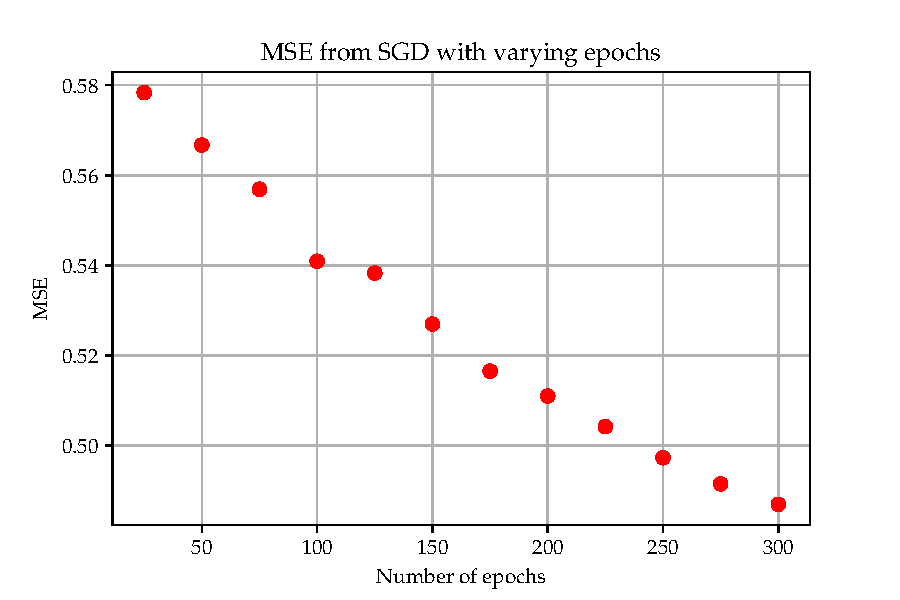
\includegraphics[width=\columnwidth]{figures/EX_A_mse_with_varying_epoch.pdf}
  \caption{\label{fig:a_mse_epoch}MSE calculated from Stochastic Gradient Descent optimization of the predictors $\theta$ as function of the number of epochs with all other hyperparameters kept fixed}
\end{figure}

The table seen in Table (\ref{tab:a_epoch_run}) shows the computational runtime associated with number of epochs.

\begin{table}
  \caption{\label{tab:a_epoch_run}Runtime in seconds computed for SGD over an increasing number of epochs}
  \begin{tabular}{|c|c|}
    \hline
    \#epochs & Runtime [s] \\ \hline
    25       & 8           \\
    50       & 17          \\
    75       & 27          \\
    100      & 38          \\
    125      & 45          \\
    150      & 57          \\
    175      & 65          \\
    200      & 80          \\
    225      & 78          \\
    250      & 79          \\
    275      & 88          \\
    300      & 95          \\
    \hline
  \end{tabular}
\end{table}

The following Figure (\ref{fig:a_bs}) plots the MSE as a function of batch\_size using the SGD algorithm in \ref{alg:sgd}.

\begin{figure}
  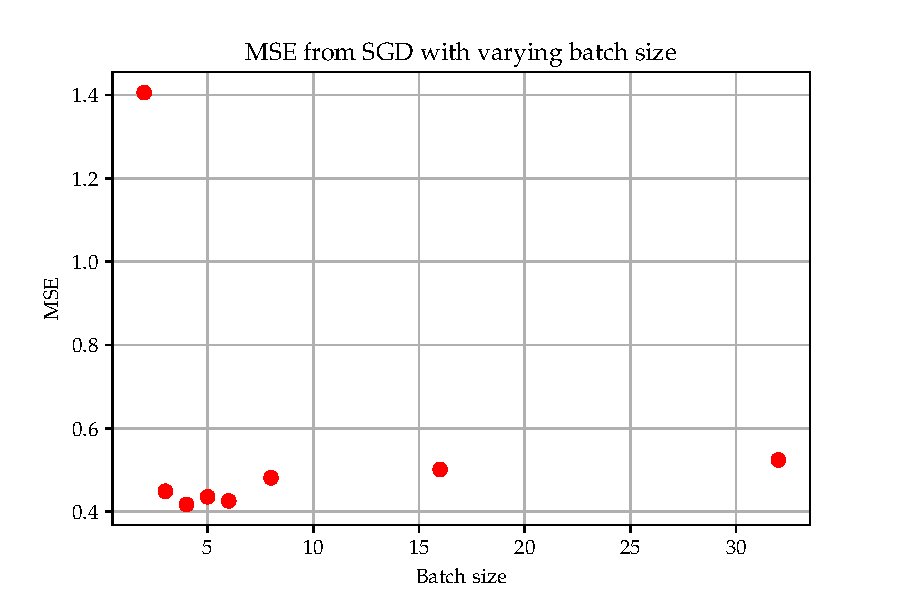
\includegraphics[width=\columnwidth]{figures/EX_A_mse_with_varying_batch_size.pdf}
  \caption{\label{fig:a_bs}MSE calculated from Stochastic Gradient Descent as function of the batch size with all other hyperparameters kept fixed}
\end{figure}

Both Figures (\ref{fig:a_gs}, \ref{fig:a_gslr}) are created using a grid search algorithm over different values of $\eta$ and $\lambda$, presented as a heatmap.

\begin{figure*}
  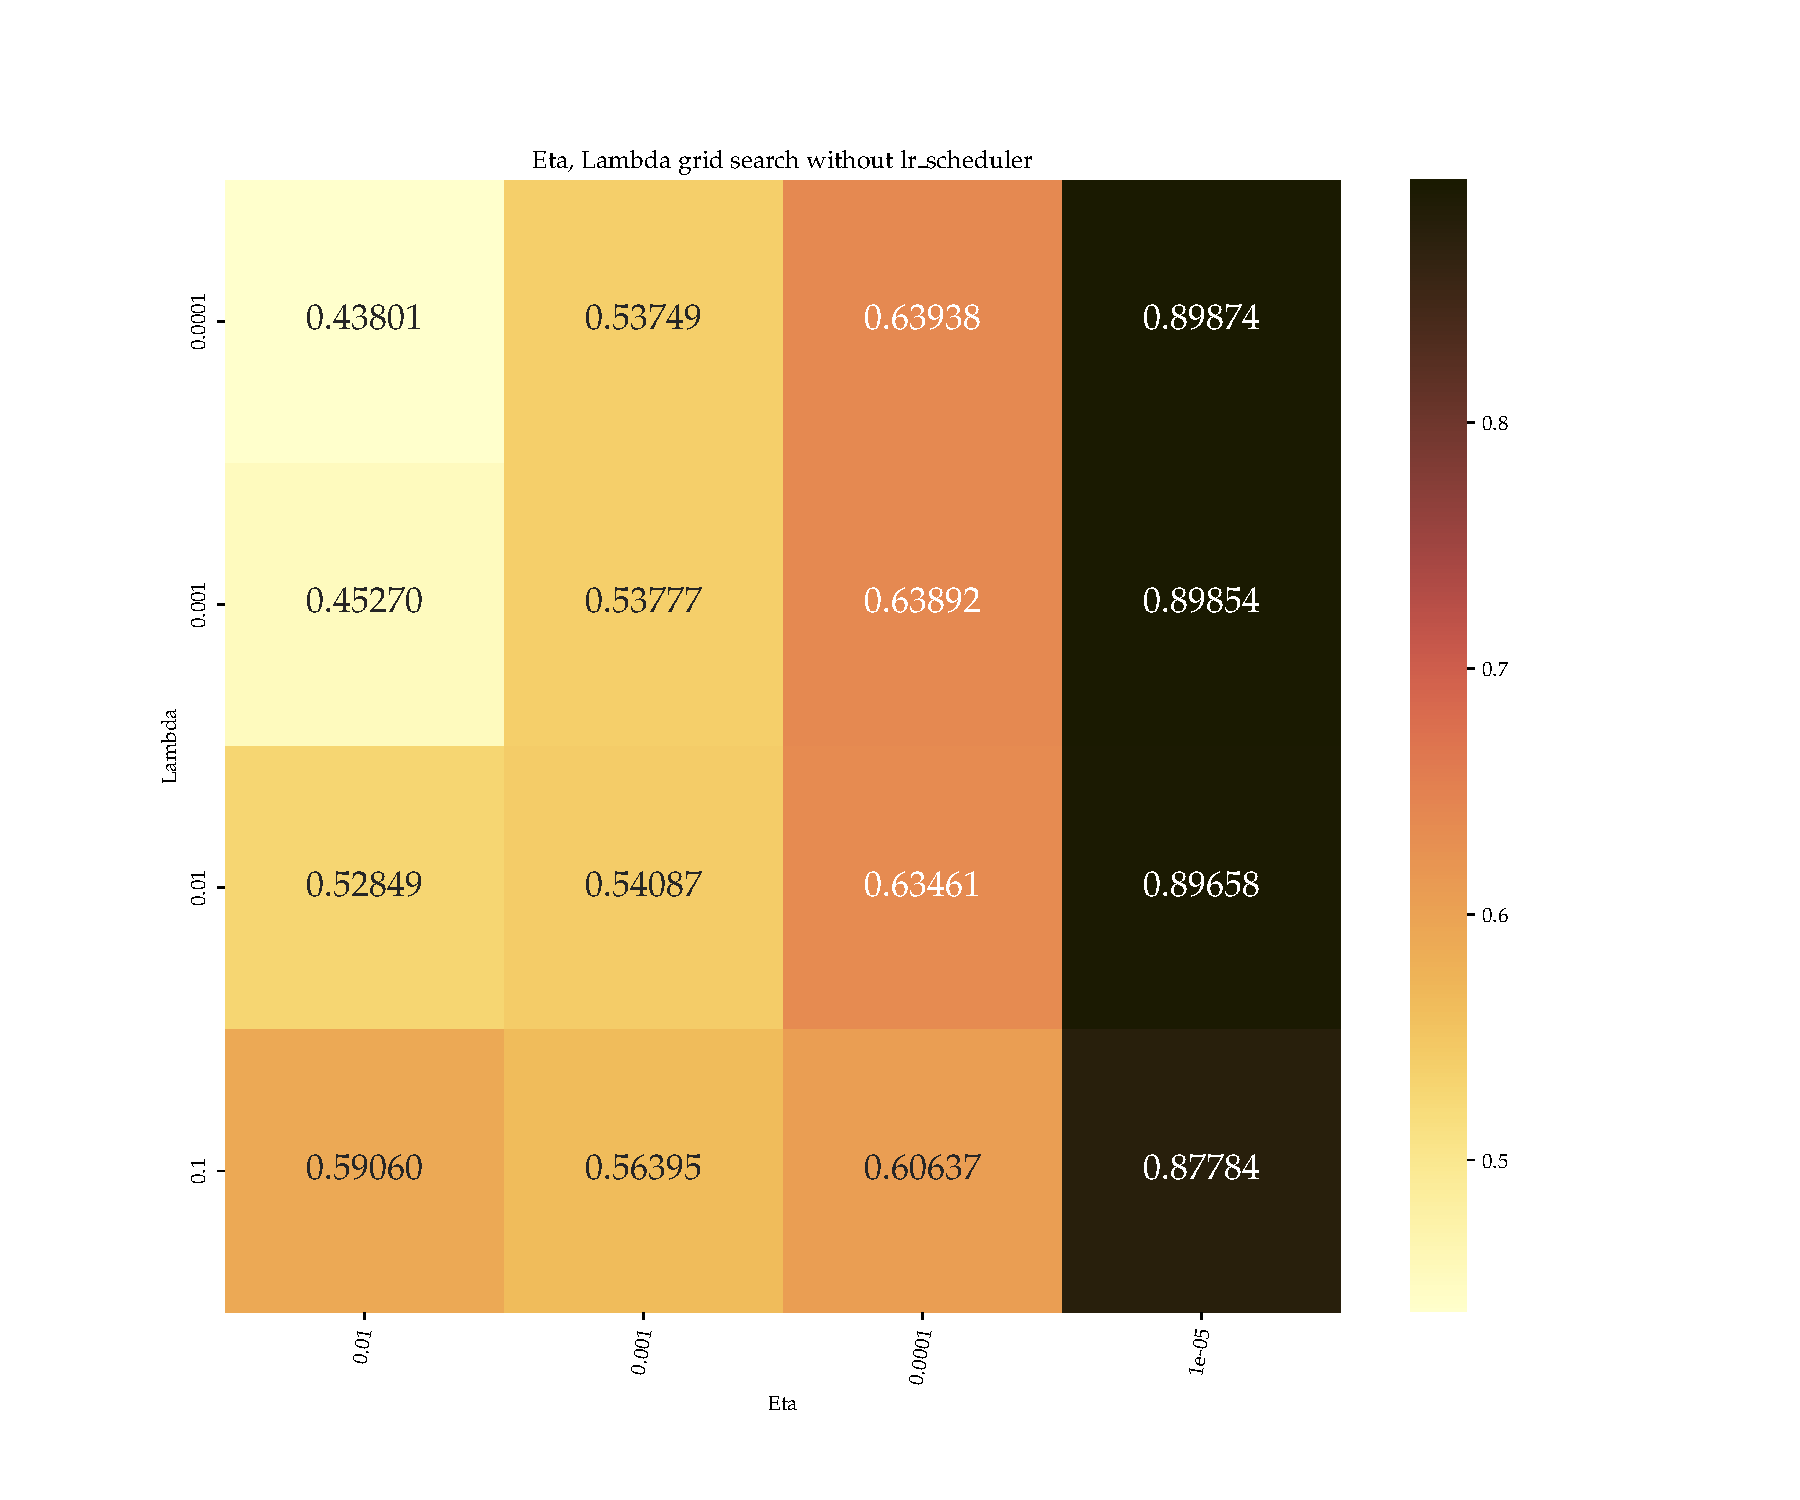
\includegraphics[width=\textwidth]{figures/EX_A__gridsearch.pdf}
  \caption{\label{fig:a_gs}MSE calculated for varying $\eta$ and $\lambda$ values in a grid search with learning rate scheduler turned off}
\end{figure*}

\begin{figure*}
  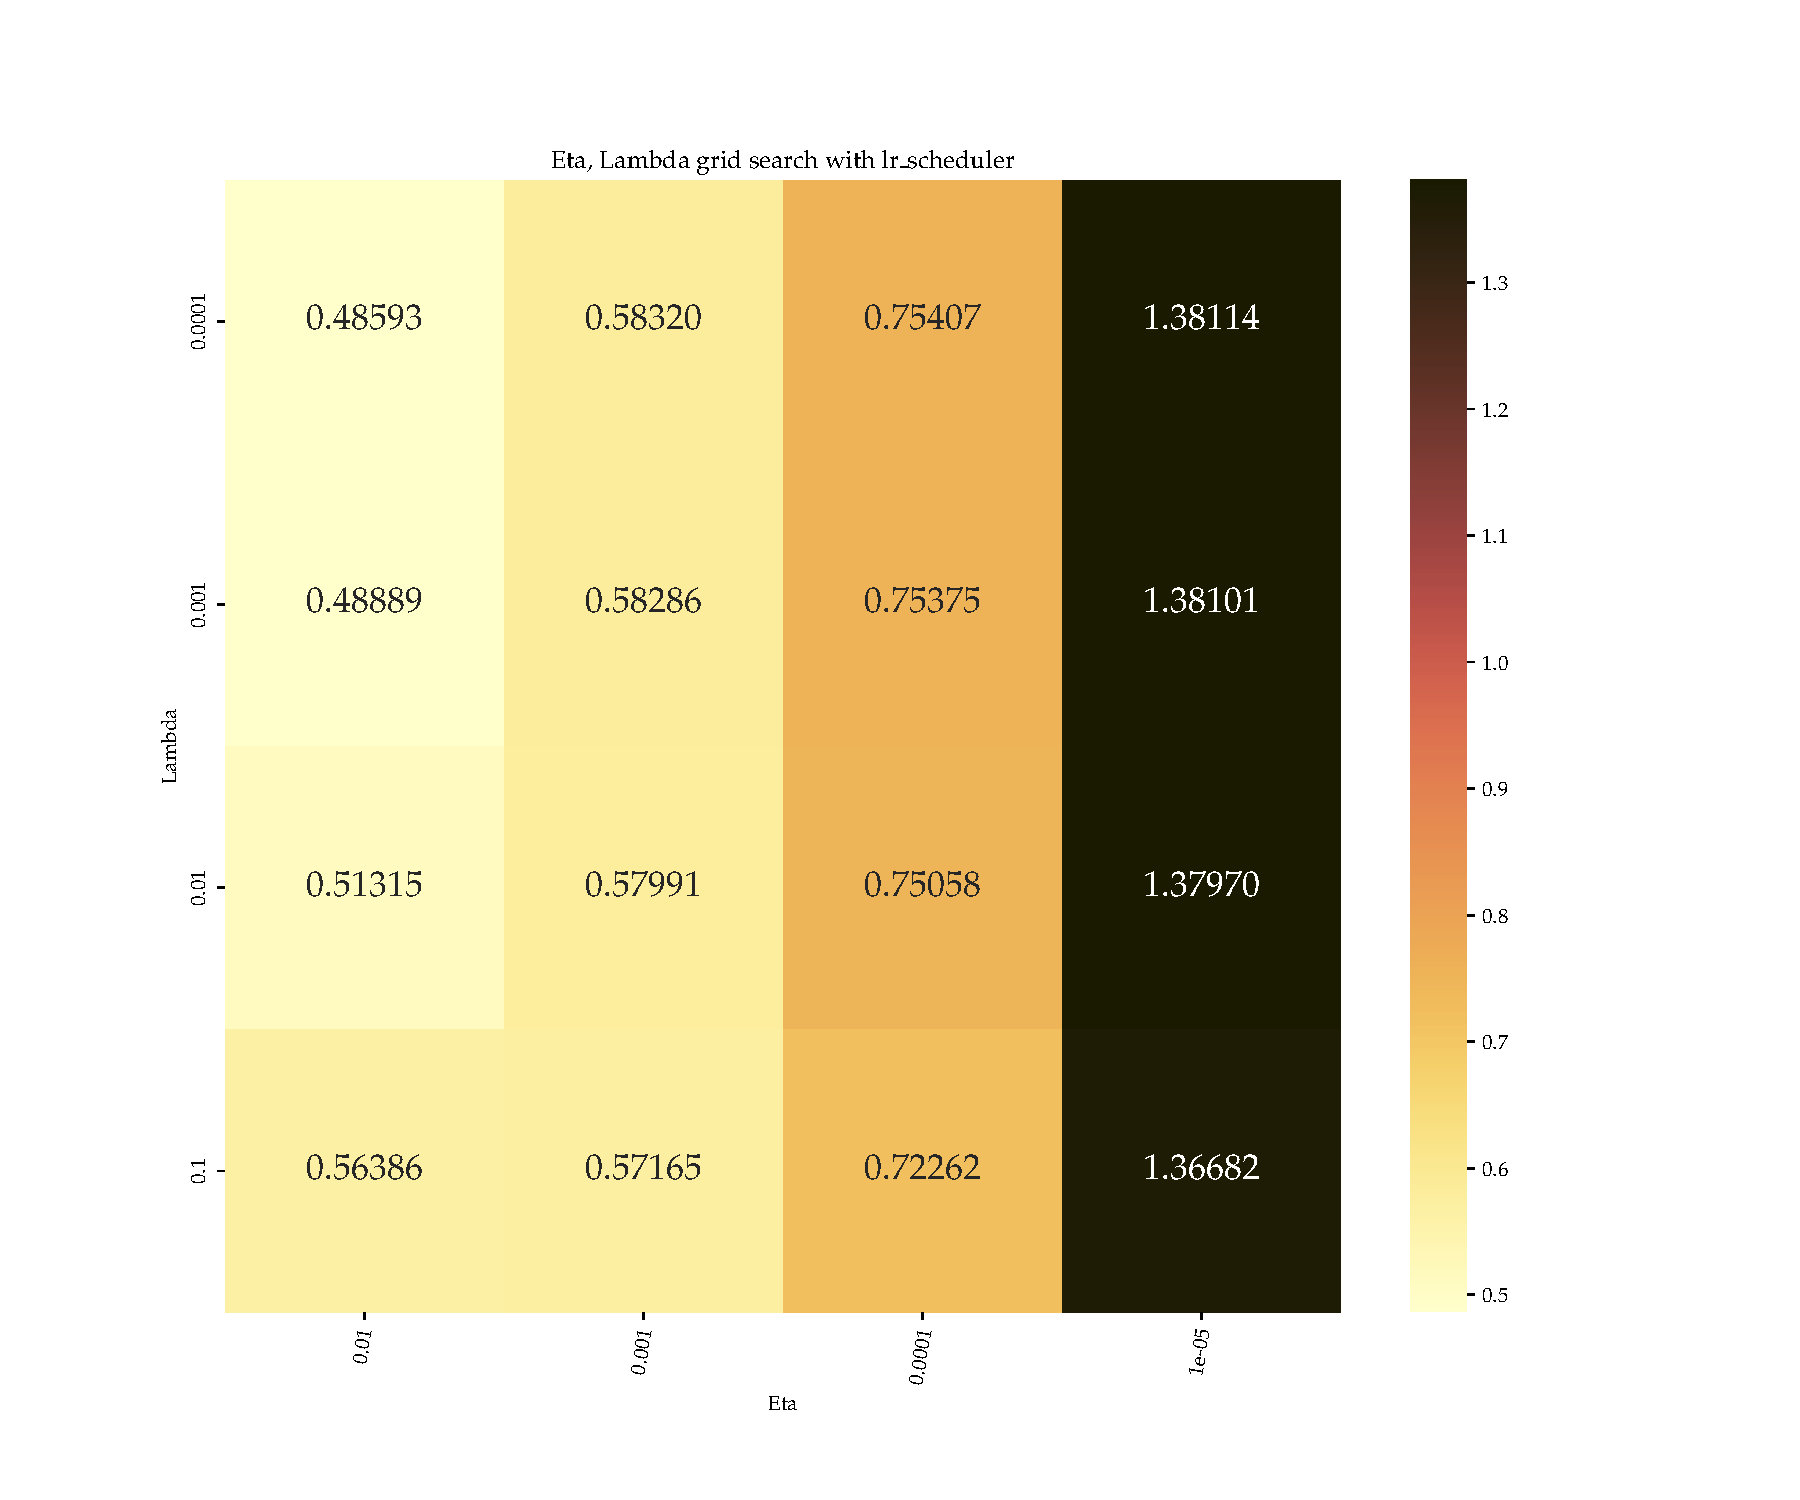
\includegraphics[width=\textwidth]{figures/EX_A__gridsearch_withlr.pdf}
  \caption{\label{fig:a_gslr}MSE calculated for varying $\eta$ and $\lambda$ values in a grid search with learning rate scheduler turned on}
\end{figure*}

Table (\ref{tab:a_mse}) displays MSE results computed from different configurations of the developed SGD algorithm, the Momentum Stochastic Gradient Descent algorithm explained in Algorithm (\ref{alg:msgd}) as well as with SGDregressor from SciKit-learn and a regression method from Project 1.

\begin{table*}
  \caption{\label{tab:a_mse}MSE values from different SGD configurations based on the optimal hyperparameters as found in the grid search}
  \begin{ruledtabular}
    \begin{tabular}{llllll}
      l2 regularizer & SGD with lr scheduler & Momentum SGD with lr scheduler & SGD w.o. lr scheduler & SciKit-learn & Regression  \\
      \hline
      Yes & 0.4783                & 0.4377                         & 0.4203                & 1.0764       & 0.3256 \\
      No & 0.4778                & 0.4354                         & 0.4171                & 1.0869       & 0.3216 \\
    \end{tabular}
  \end{ruledtabular}
\end{table*}

\subsection{Regression}
Our Neural Network has been implemented with the Feed Forward pass and Backpropagation algorithm as described in Algorithm (\ref{alg:ff}) and (\ref{alg:bp}). Moreover, different model architecture has been implemented following the design of Figure (\ref{fig:small_architecture}) and (\ref{fig:large_architecture}). 

Figure (\ref{fig:leaky_relu_NN_vs_tf}) display a grid search over different learning rate $\eta$ and regularization terms $\lambda$ for a model with the Leaky ReLU activation function and large model architecture for both our Neural Network and the TensorFlow implementation.

\begin{figure*}
  \vspace*{-2.5cm}
  \subfloat[Own NN model - Showing number of parameters, $\eta$ and $\lambda$\label{fig:gridsearch_leaky_relu_NN_best}]{
    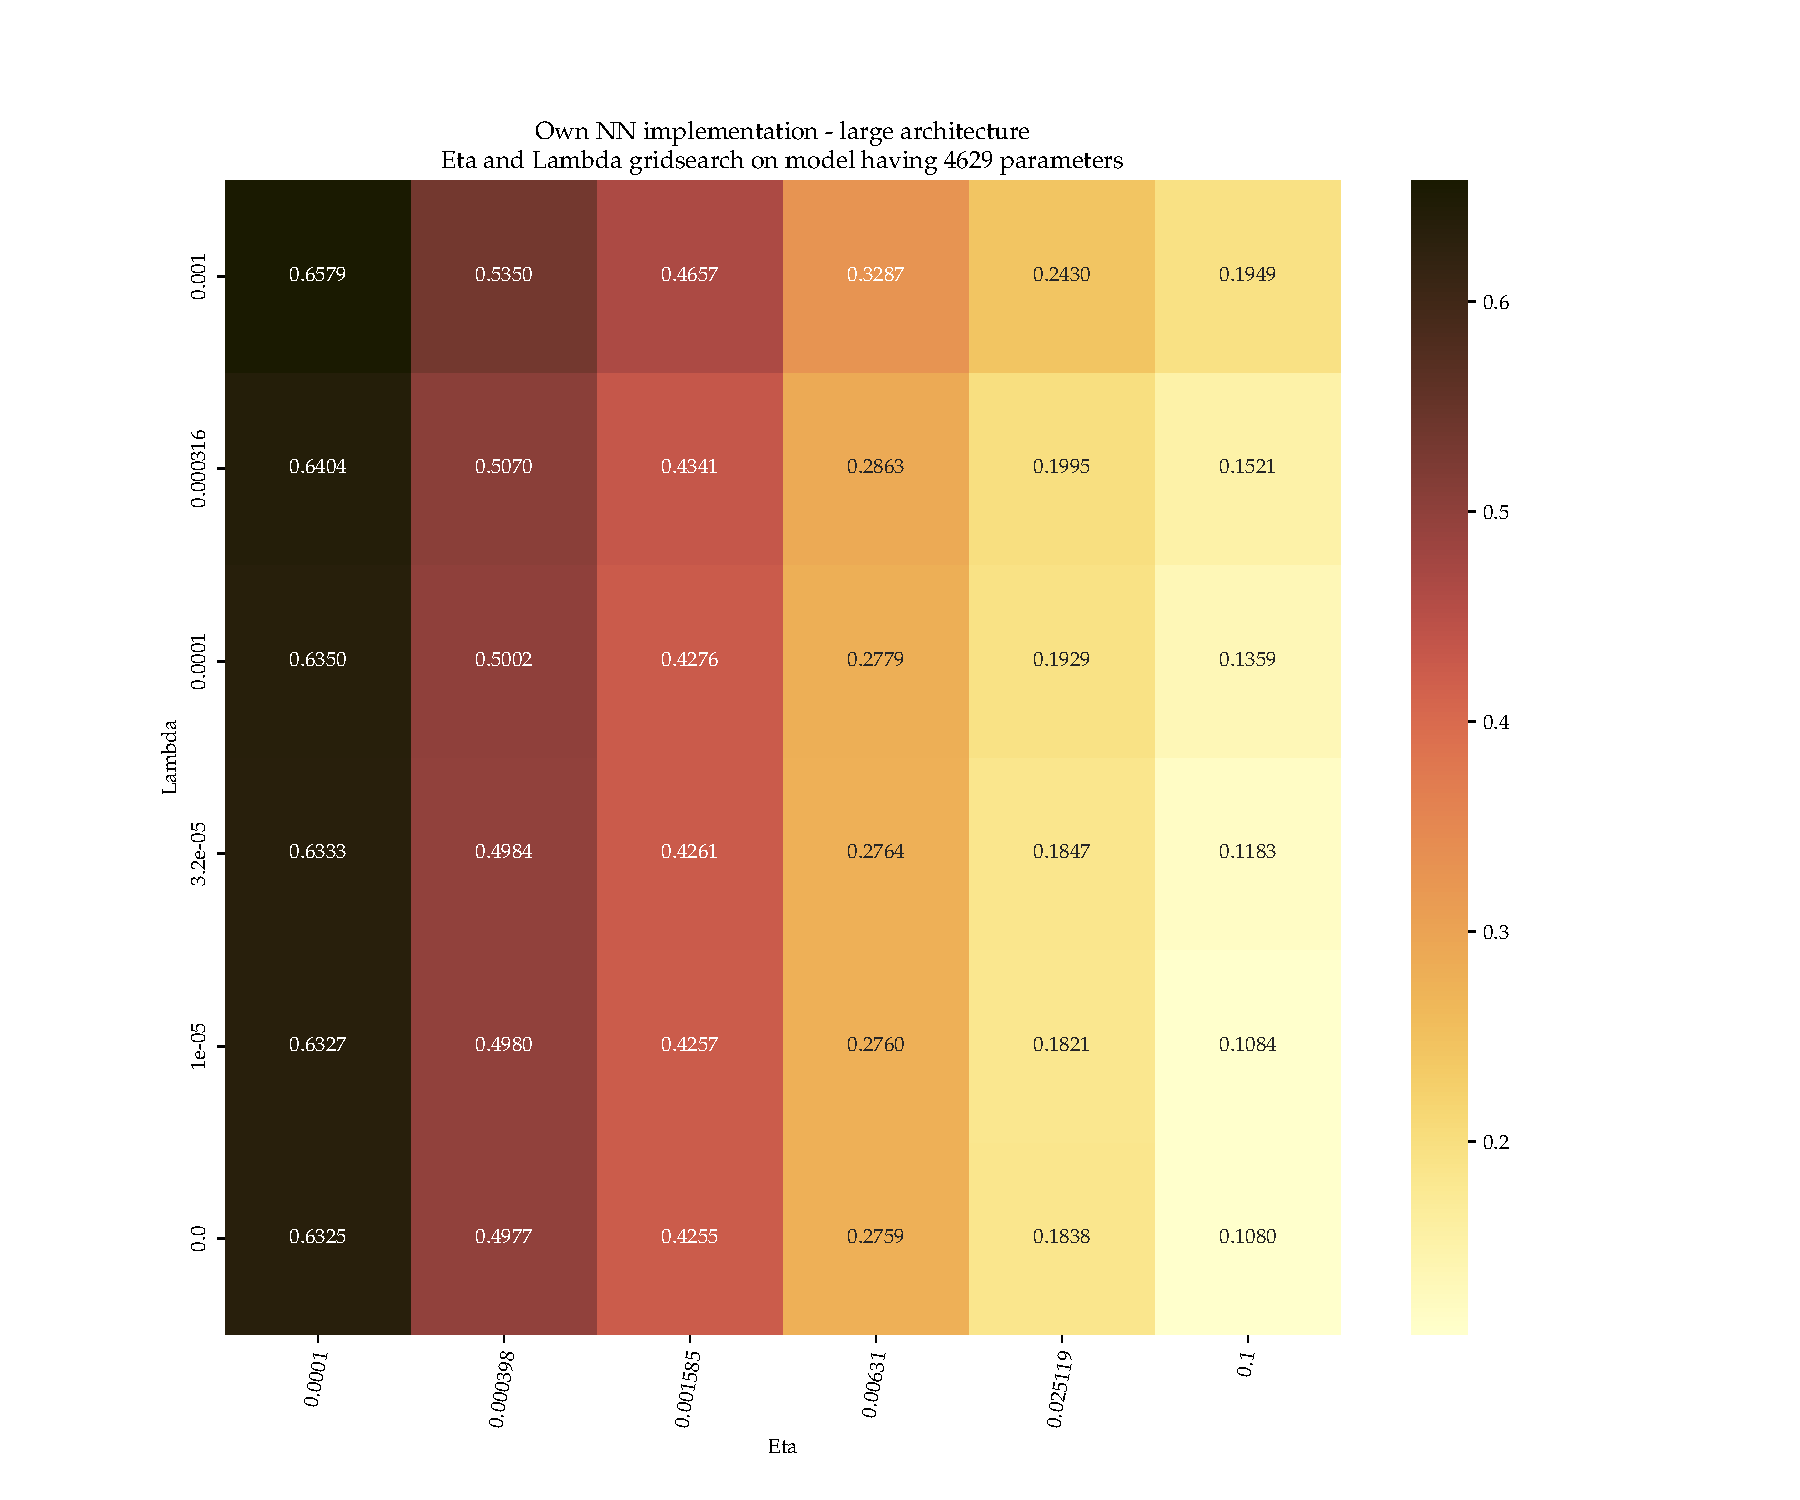
\includegraphics[width=.89\textwidth]{figures/EX_C_heatmap_own_NN_large_parameters_4629_leaky_relu.pdf}
  }\\
  \vspace*{-0.45cm}
  \subfloat[Tensorflow model - Showing number of parameters, $\eta$ and $\lambda$\label{fig:gridsearch_leaky_relu_TF_best}]{
    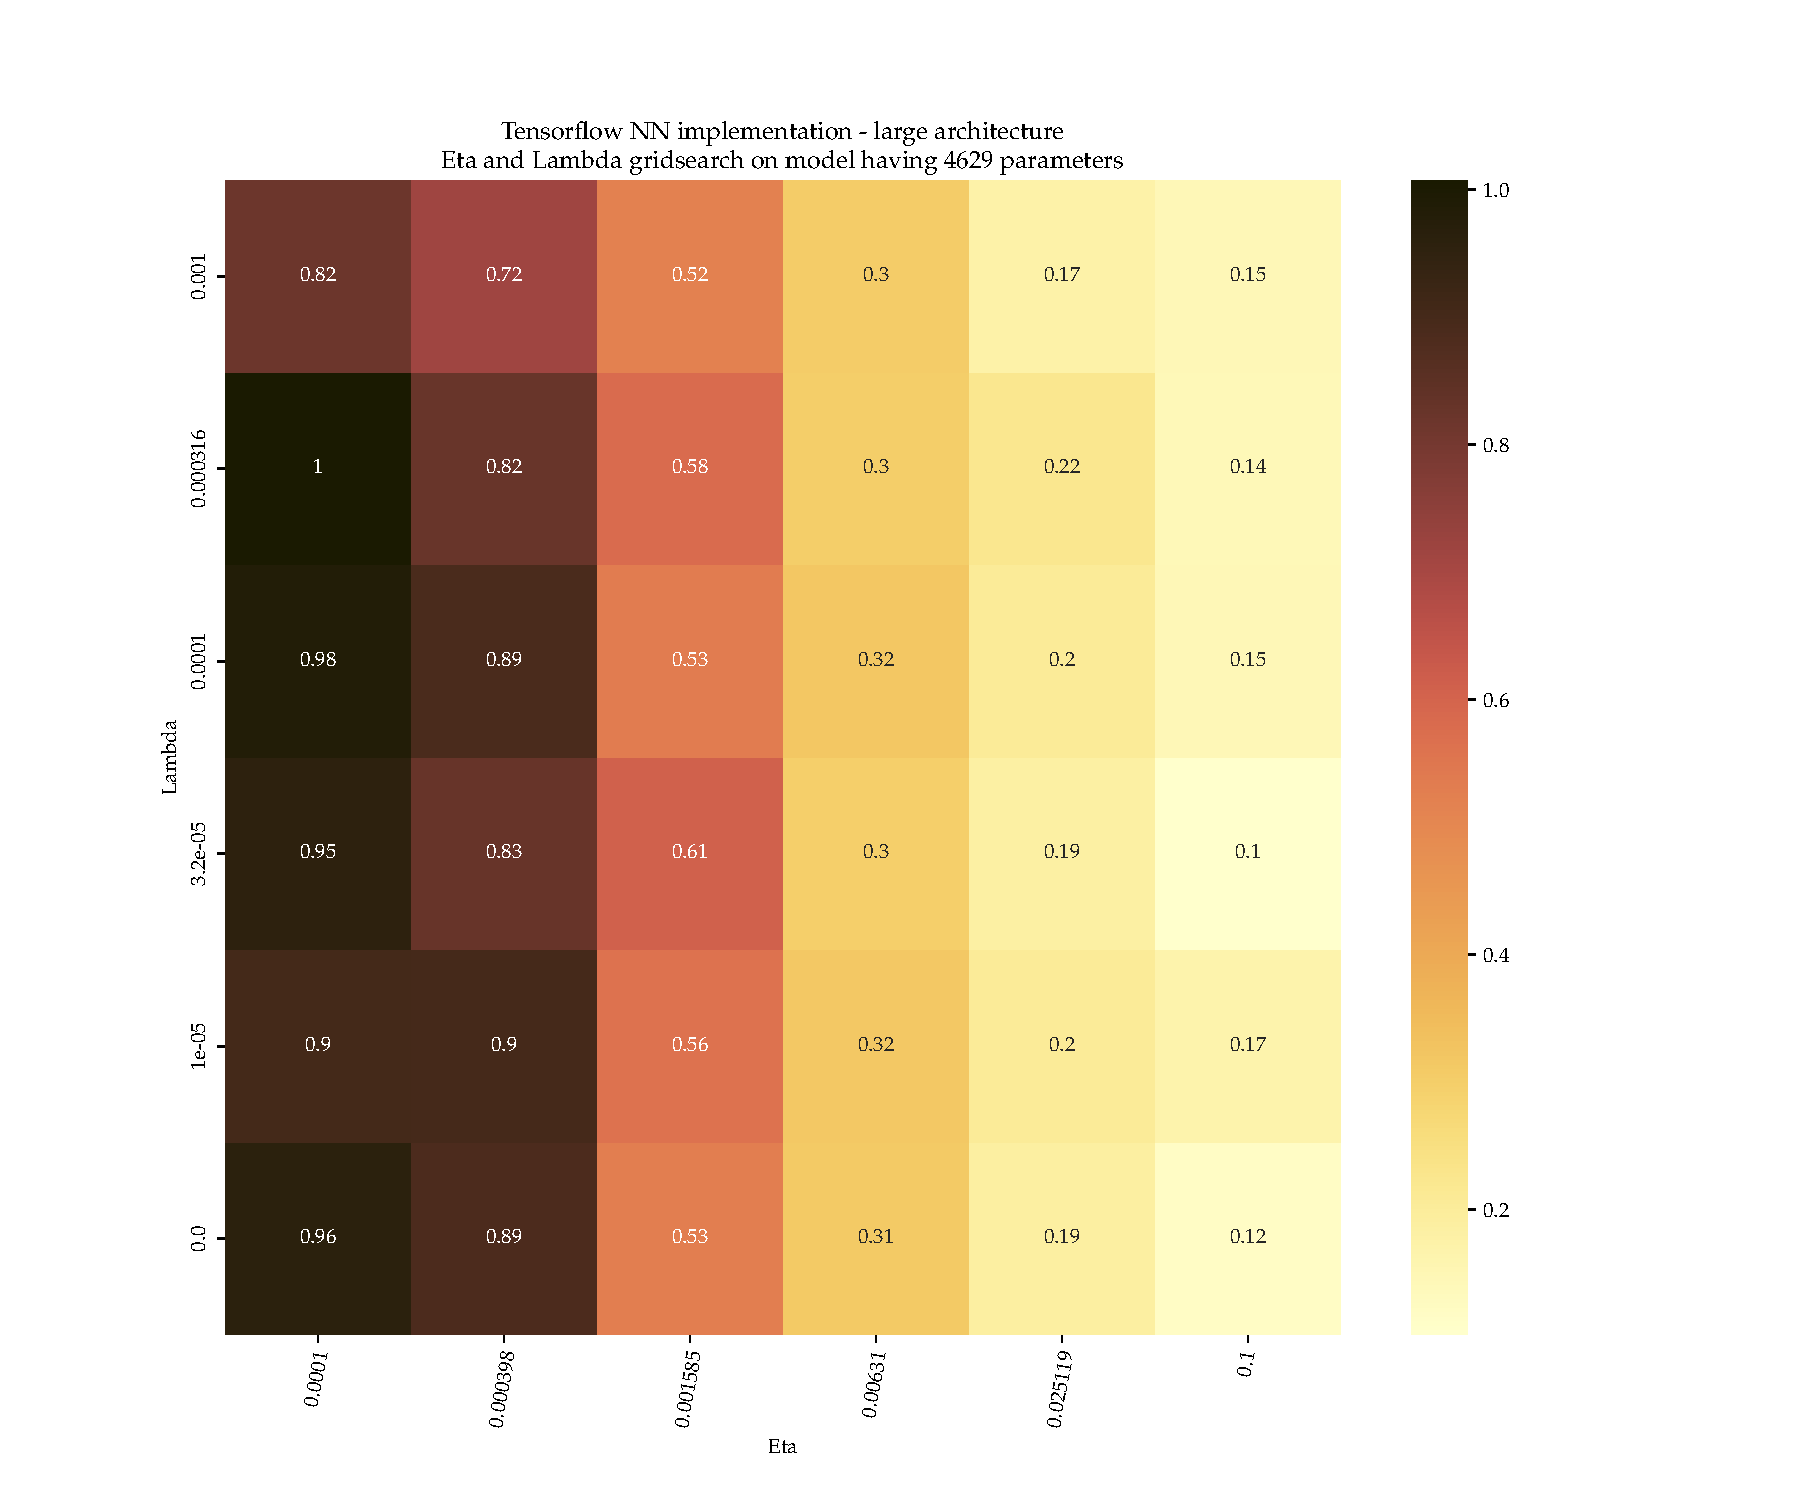
\includegraphics[width=.89\textwidth]{figures/EX_C_heatmap_tf_large_parameters_4629_leaky_relu.pdf}
  }
  \caption{Grid search visualized for the best parameters using Leaky RELU activation function\label{fig:leaky_relu_NN_vs_tf}}
\end{figure*}


Moreover, Figure (\ref{fig:NN_model_complexity}) plots output MSE for three different models with different activation functions as a dependency on the number of parameters in the model.
\begin{figure}
  \subfloat{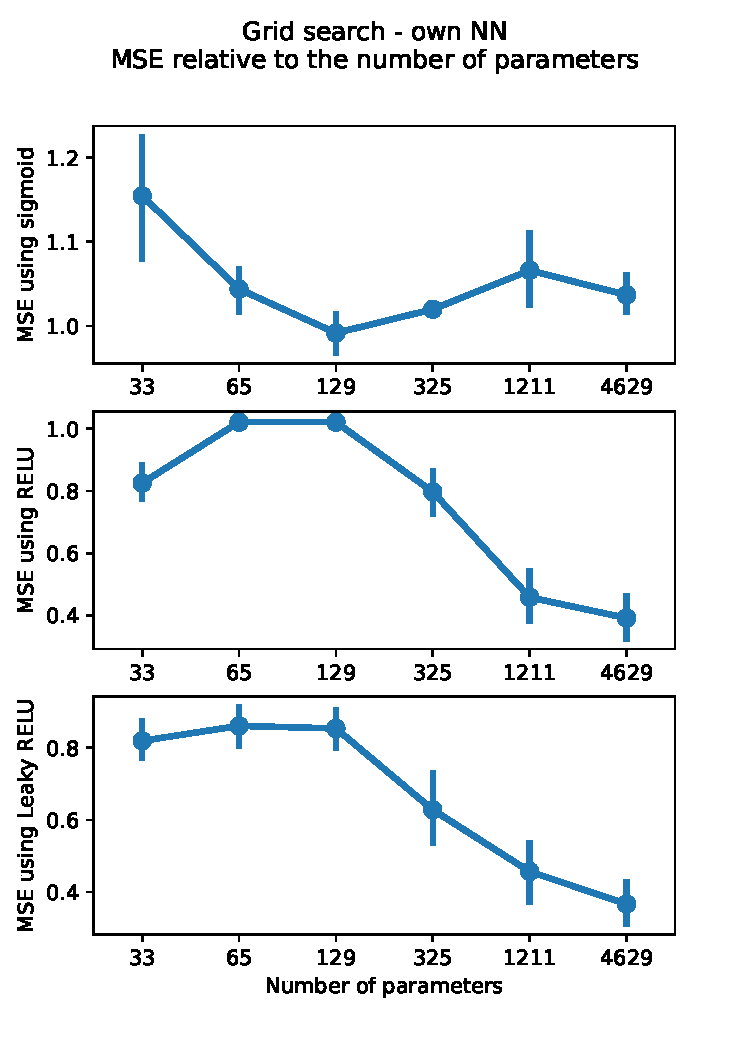
\includegraphics[width=\columnwidth]{figures/NN_MSE_vs_Parameters.pdf}}
  \caption{MSE score vs number of paramteters in model architecture. Vertical lines visualize the minimum and maximum MSE value obtained using gridsearch over $\eta$ and $\lambda$ with respect to the current model architecture\label{fig:NN_model_complexity}}
\end{figure}


Figure (\ref{fig:small_vs_large_architecture_training}) plots the different model architectures and activation function dependance on number of epochs. 
\begin{figure*}
  \subfloat[Best fitted NN model using sigmoid and small arhitecture\label{fig:small_sigmoid_training}]{
    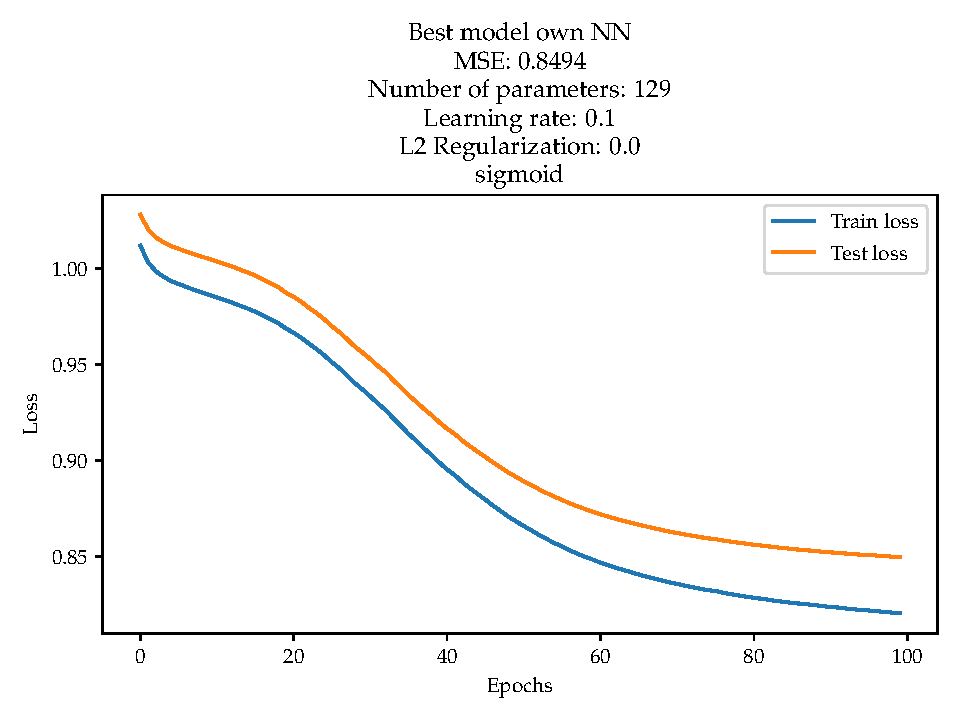
\includegraphics[width=.5\textwidth]{figures/EX_B_own_NN_best_training_small_sigmoid_lr_0.1.pdf}
  }
  \subfloat[Best fitted NN model using sigmoid and large arhitecture\label{fig:large_sigmoid_training}]{
    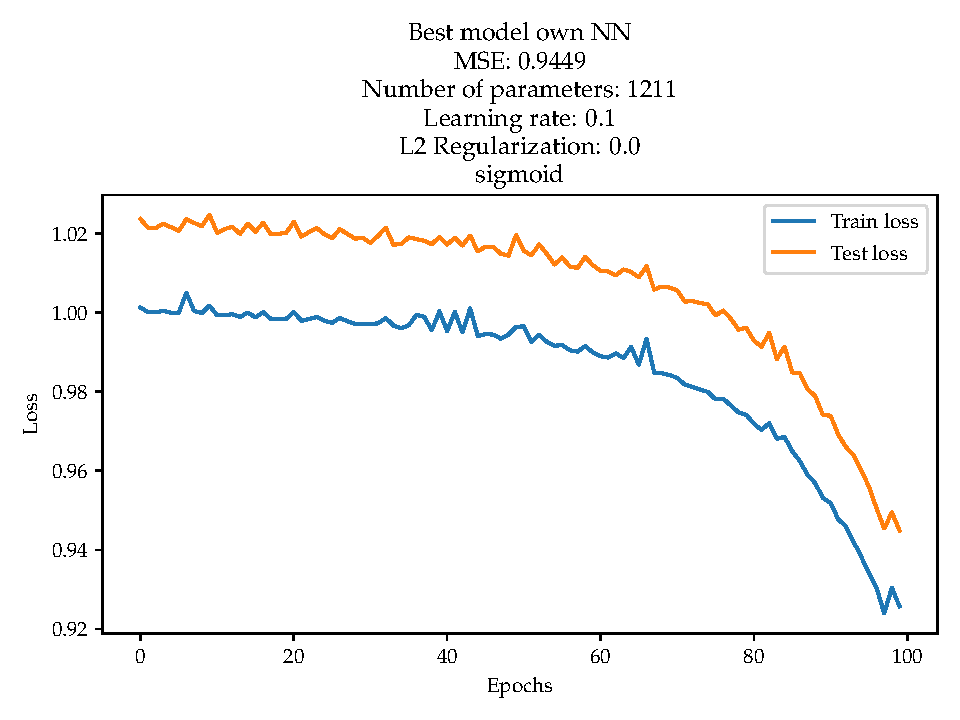
\includegraphics[width=.5\textwidth]{figures/EX_B_own_NN_best_training_large_sigmoid_lr_0.1.pdf}
  }\\
  \subfloat[Best fitted NN model using RELU and small arhitecture\label{fig:small_relu_training}]{
    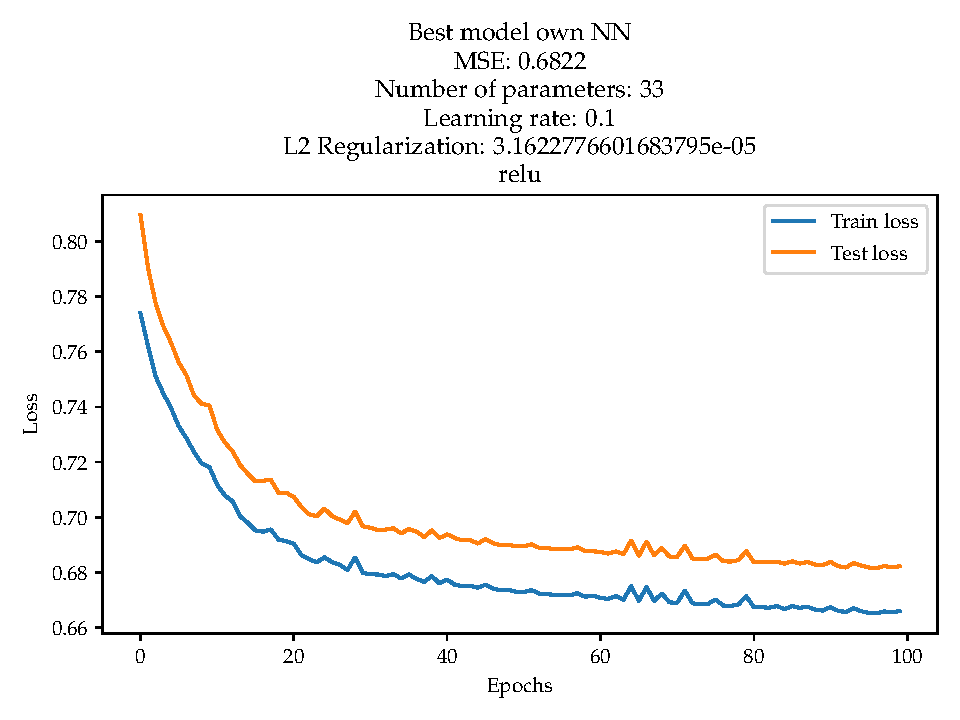
\includegraphics[width=.5\textwidth]{figures/EX_C_own_NN_best_training_small_relu_lr_0.1.pdf}
  }
  \subfloat[Best fitted NN model using RELU and large arhitecture\label{fig:large_relu_training}]{
    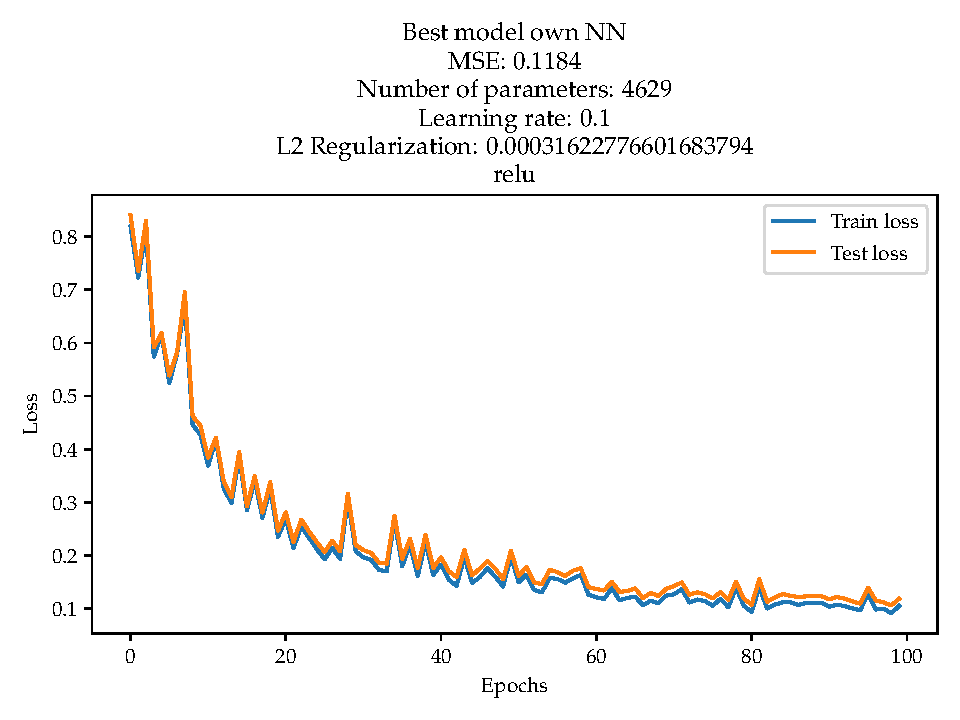
\includegraphics[width=.5\textwidth]{figures/EX_C_own_NN_best_training_large_relu_lr_0.1.pdf}
  }\\
  \subfloat[Best fitted NN model using Leaky RELU and small arhitecture\label{fig:small_leaky_relu_training}]{
    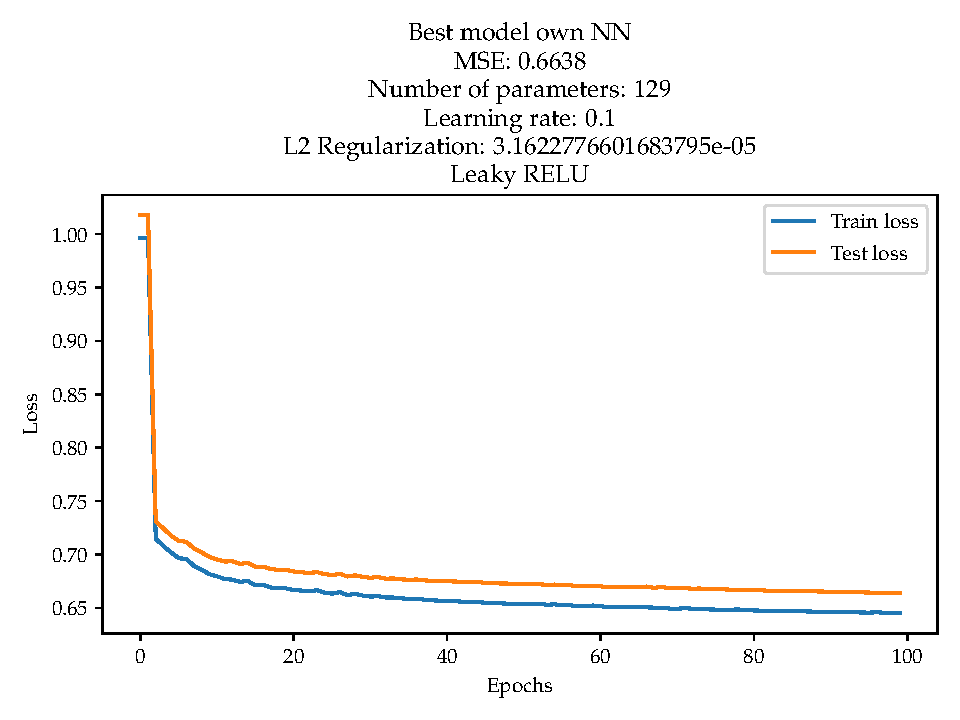
\includegraphics[width=.5\textwidth]{figures/EX_C_own_NN_best_training_small_leaky_relu_lr_0.1.pdf}
  }
  \subfloat[Best fitted NN model using Leaky RELU large arhitecture\label{fig:large_leaky_relu_training}]{
    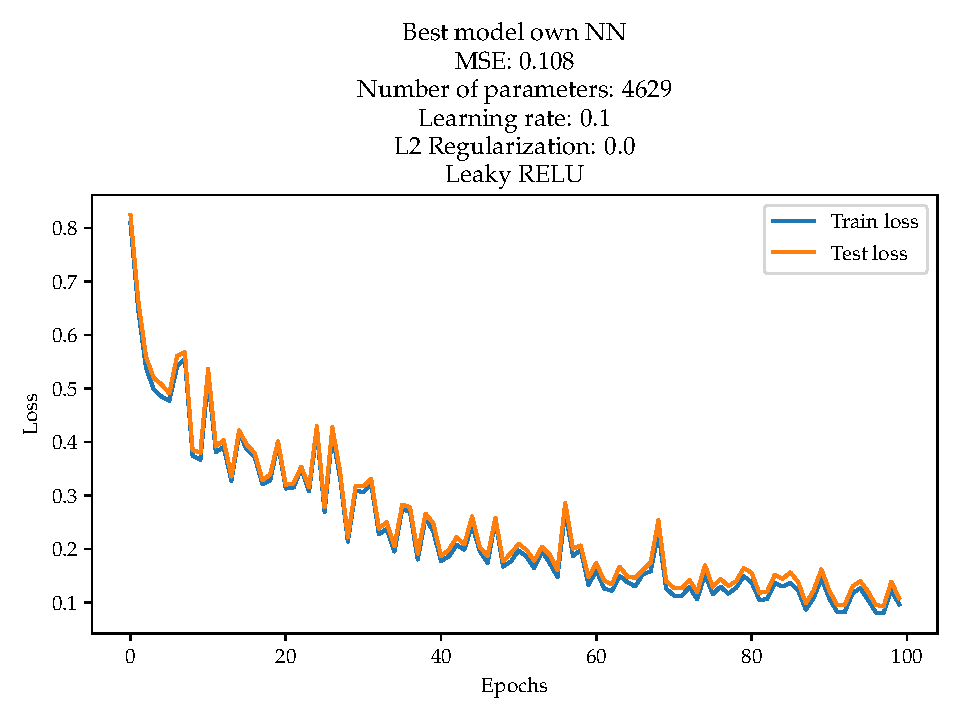
\includegraphics[width=.5\textwidth]{figures/EX_C_own_NN_best_training_large_leaky_relu_lr_0.1.pdf}
  }
  \caption{MSE computed for small and large model architecture for the different activation functions as a function of epochs\label{fig:small_vs_large_architecture_training}}
\end{figure*}

Table (\ref{tab:grid_search_optimal_sigmoid} - \ref{tab:grid_search_optimal_Leaky_RELU}) display the optimal hyperparamter setup as we have found for a model of each activation function.
\begin{table}
  \caption{\label{tab:grid_search_optimal_sigmoid}Optimal grid search parameters for the sigmoid activation function}
  \csvautotabular{data/report_data/NN_optimal_parameters_small_sigmoid.csv}
\end{table}

\begin{table}
  \caption{\label{tab:grid_search_optimal_RELU}Optimal grid search parameters for the RELU activation function}
  \csvautotabular{data/report_data/NN_optimal_parameters_large_relu.csv}
\end{table}

\begin{table}
  \caption{\label{tab:grid_search_optimal_Leaky_RELU}Optimal grid search parameters for the Leaky RELU activation function}
  \csvautotabular{data/report_data/NN_optimal_parameters_large_leaky_relu.csv}
\end{table}

Figure (\ref{fig:own_NN_vs_tf}) plots both our own Neural Network as well as the implementation using TensorFlow with the Leaky ReLU activation function with found optimal architecture as a function of number of epochs.
\begin{figure*}
  \hspace*{-1.5cm}
  \subfloat{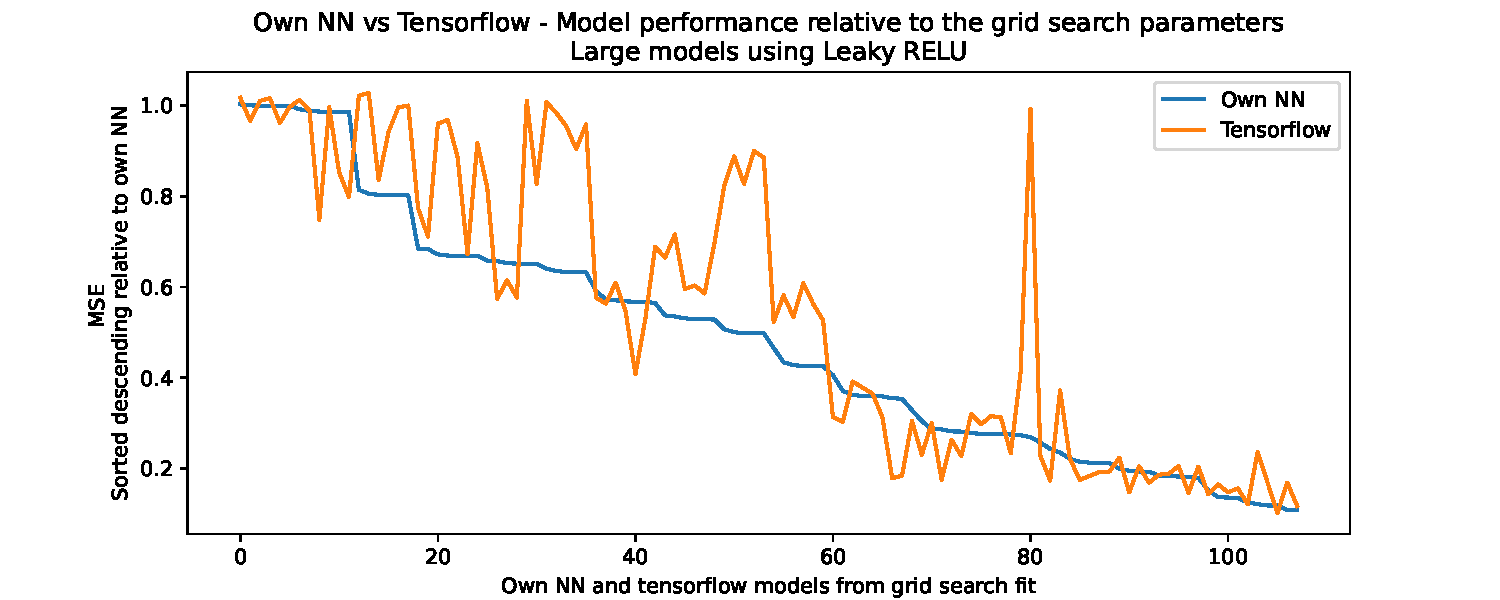
\includegraphics[width=1.1\textwidth]{figures/Own_NN_vs_Tensorflow_Leaky_RELU_Large_architecture.pdf}}
  \caption{MSE comparison between own NN and Tensorflow - MSE from grid search using Leaky RELU\label{fig:own_NN_vs_tf}}
\end{figure*}

We have visualized our terrain reconstruction in both Figure (\ref{fig:2D_preds_NN_vs_OLS}) and (\ref{fig:3D_preds_NN_vs_OLS}). Both reconstructions were made using the optimal model architecture for our Neural Network. Moreover, for comparison, the best result from Project 1 using OLS with max polynomial degree 10 is shown.
\begin{figure*}
  \subfloat{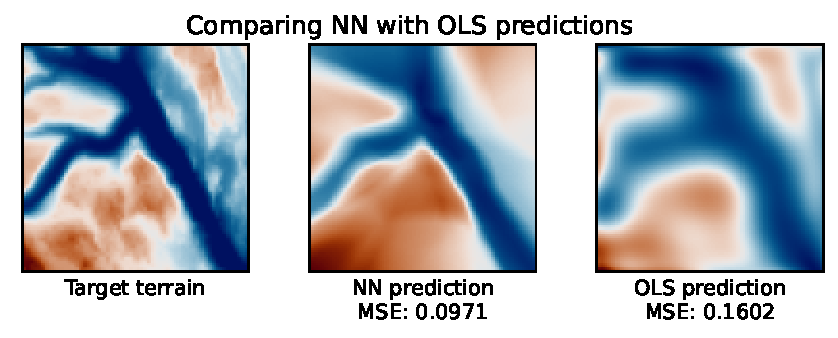
\includegraphics[width=1.0\textwidth]{figures/NN_vs_OLS_2D.pdf}}
  \caption{2D prediction comparison between own NN and own OLS \label{fig:2D_preds_NN_vs_OLS}}
\end{figure*}

\begin{figure*}
  \subfloat{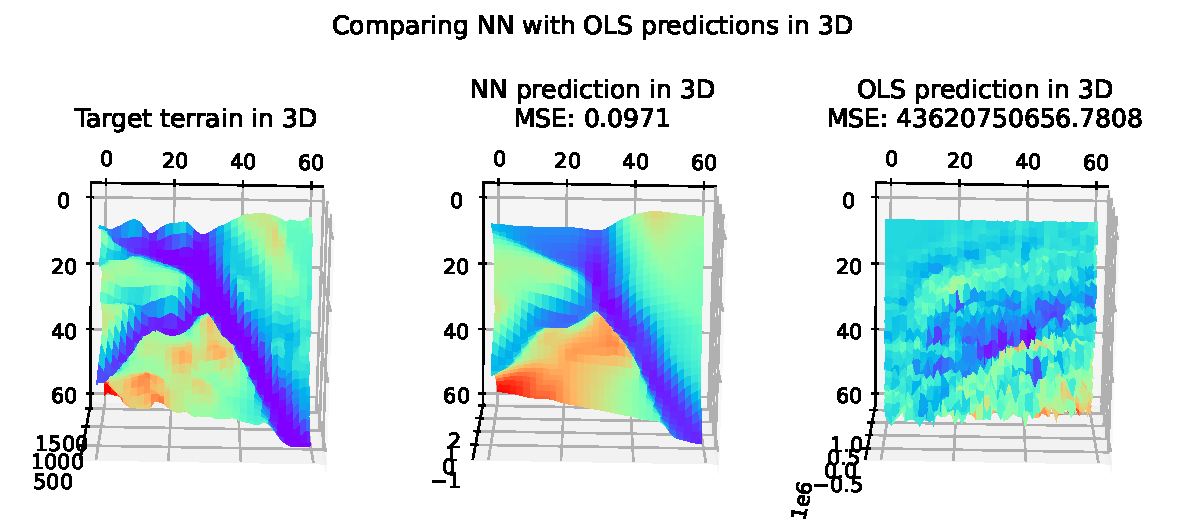
\includegraphics[width=1.0\textwidth]{figures/NN_vs_OLS_3D.pdf}}
  \caption{3D prediction comparison between own NN and own OLS \label{fig:3D_preds_NN_vs_OLS}}
\end{figure*}


Table (\ref{tab:cross_val_scores}) shows a 7 fold cross validation of the optimal model, though with the learning rate $\eta = 0.05$. 
\begin{table}
  \caption{\label{tab:cross_val_scores}MSE from 7-fold cross-validation on the regression problem with $\eta = 0.05$ as only changed hyperparameter from the optimal architecture}
  \csvautotabular{data/report_data/EX_C_cross_val.csv}
\end{table}

\subsection{Classification}

For the classification problem, we used our Neural Network following the three changes mentioned in the prior Section. Figure (\ref{fig:conf_matrix_home_torch}) plots the Confusion matrices for both the own Neural Network classifier and the similar PyTorch classifier. Both confusion matrices are created from models using optimal parameters as found doing a grid search (not shown).

\begin{figure*}
  \subfloat[Own NN model - Confusion Matrix\label{fig:EX_D_homebrew_conf_matrix_a}]{
    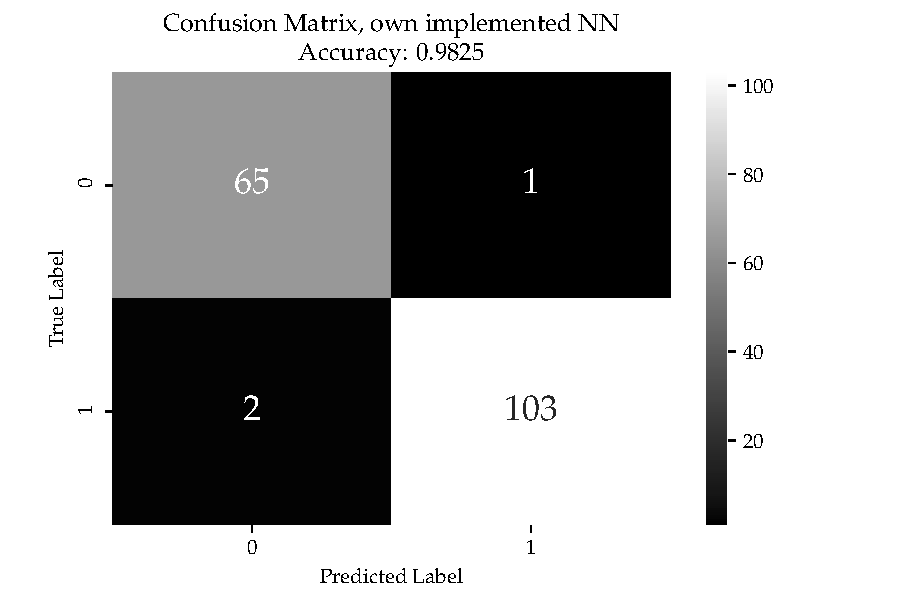
\includegraphics[width=\columnwidth]{figures/EX_D_homebrew_conf_matrix.pdf}
  }
  \subfloat[PyTorch model - Confusion Matrix\label{fig:EX_D_torch_conf_matrix_b}]{
    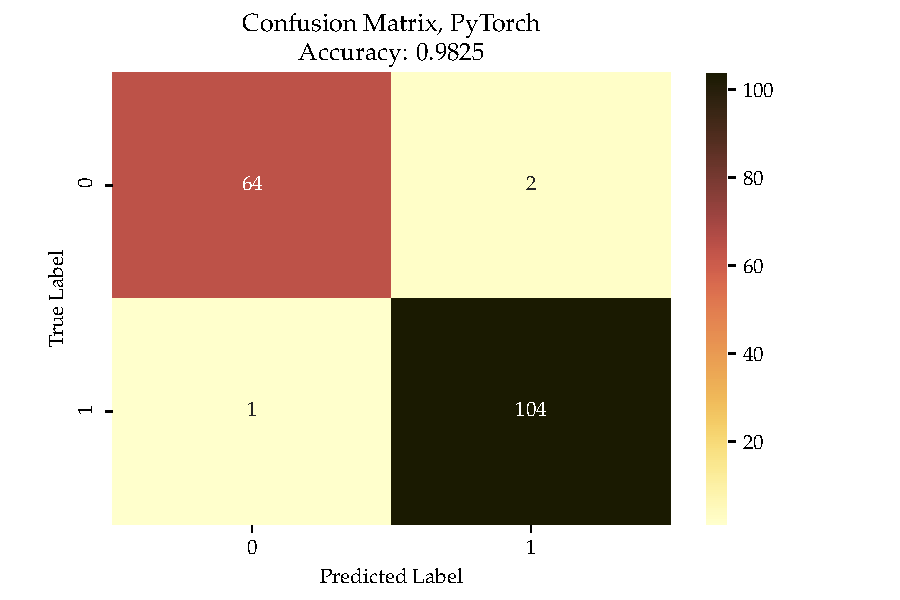
\includegraphics[width=\columnwidth]{figures/EX_D_torch_conf_matrix.pdf}
  }
  \caption{Confusion matrices for our own Neural Network as well as a similar Neural Network implemented using PyTorch. Both Neural Networks has been initialized using parameters found from independent Grid Searches.\label{fig:conf_matrix_home_torch}}
\end{figure*}

Figure (\ref{fig:EX_E_logreg_gridsearch}) shows the result of a grid search over different values of $\eta$ and $\lambda$ for the Logistic Regression with Stochastic Gradient Descent.
\begin{figure*}
  \subfloat{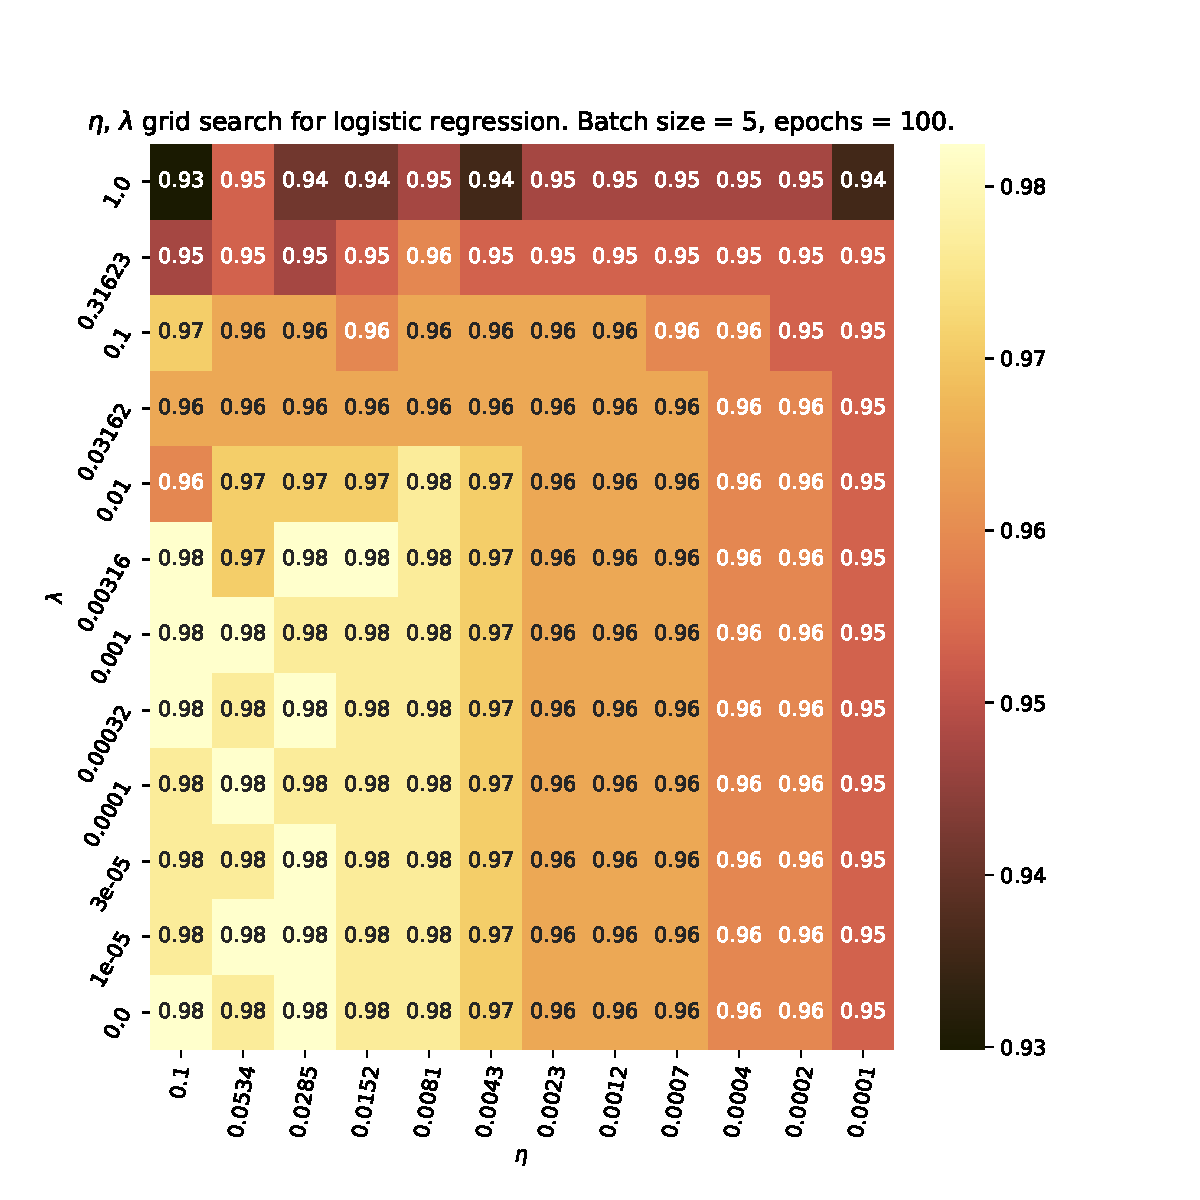
\includegraphics[width=1.0\textwidth]{figures/EX_E_logreg_gridsearch.pdf}}
  \caption{Grid search accuracies for logistic regression with varying $\eta$, $\lambda$ values. \label{fig:EX_E_logreg_gridsearch}}
\end{figure*}

Moreover, Figure (\ref{fig:conf_matrix_sgd_nrm}) also plots confusion matrices, though for two different Logistic Regression models. Namely Stochastic Gradient Descent and Newton Raphson. For the SGD Logistic Regression, the hyperparameters has been optimized according to the grid search in Figure (\ref{fig:EX_E_logreg_gridsearch}).

\begin{figure*}
  \subfloat[Logistic Regression with NRM - Confusion Matrix\label{fig:EX_E_logreg_nrm_confmat_a}]{
    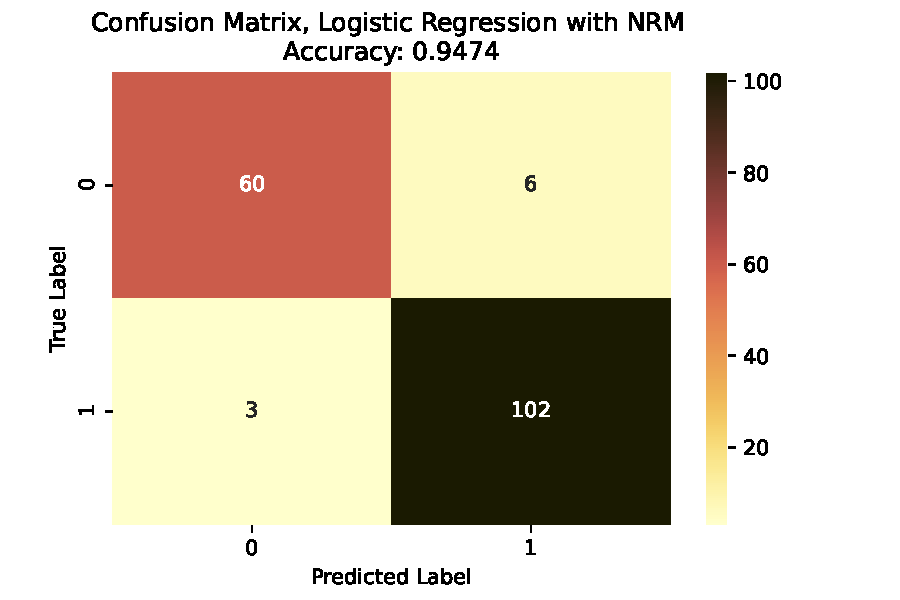
\includegraphics[width=\columnwidth]{figures/EX_E_logreg_nrm_confmat.pdf}
  }
  \subfloat[Logistic Regression with SGD - Confusion Matrix\label{fig:EX_E_logreg_sgd_confmat_b}]{
    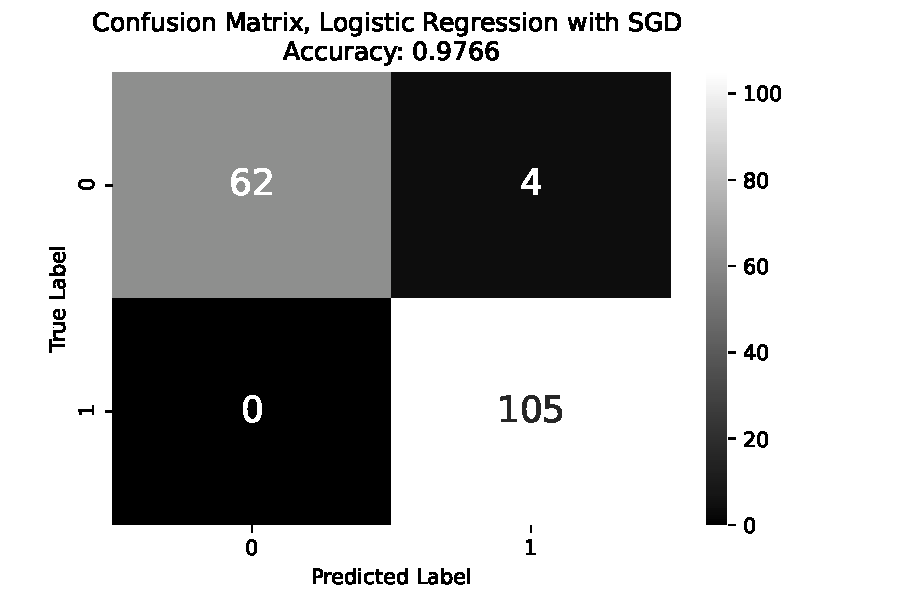
\includegraphics[width=\columnwidth]{figures/EX_E_logreg_sgd_confmat.pdf}
  }
  \caption{Confusion matrices for Logistic Regression using both Stochastic Gradient Descent and Newton Raphson. The parameters for the Logistic Regression has been optimized considering the SGD algorithm using the Grid Search. Newton Raphson does not require the same hyperparameters.\label{fig:conf_matrix_sgd_nrm}}
\end{figure*}

The plot shown in Figure (\ref{fig:EX_E_roc_curve}) is a Receiver Operating Characteristic plot with curves for the different classification algorithms used in this Project.
\begin{figure}
  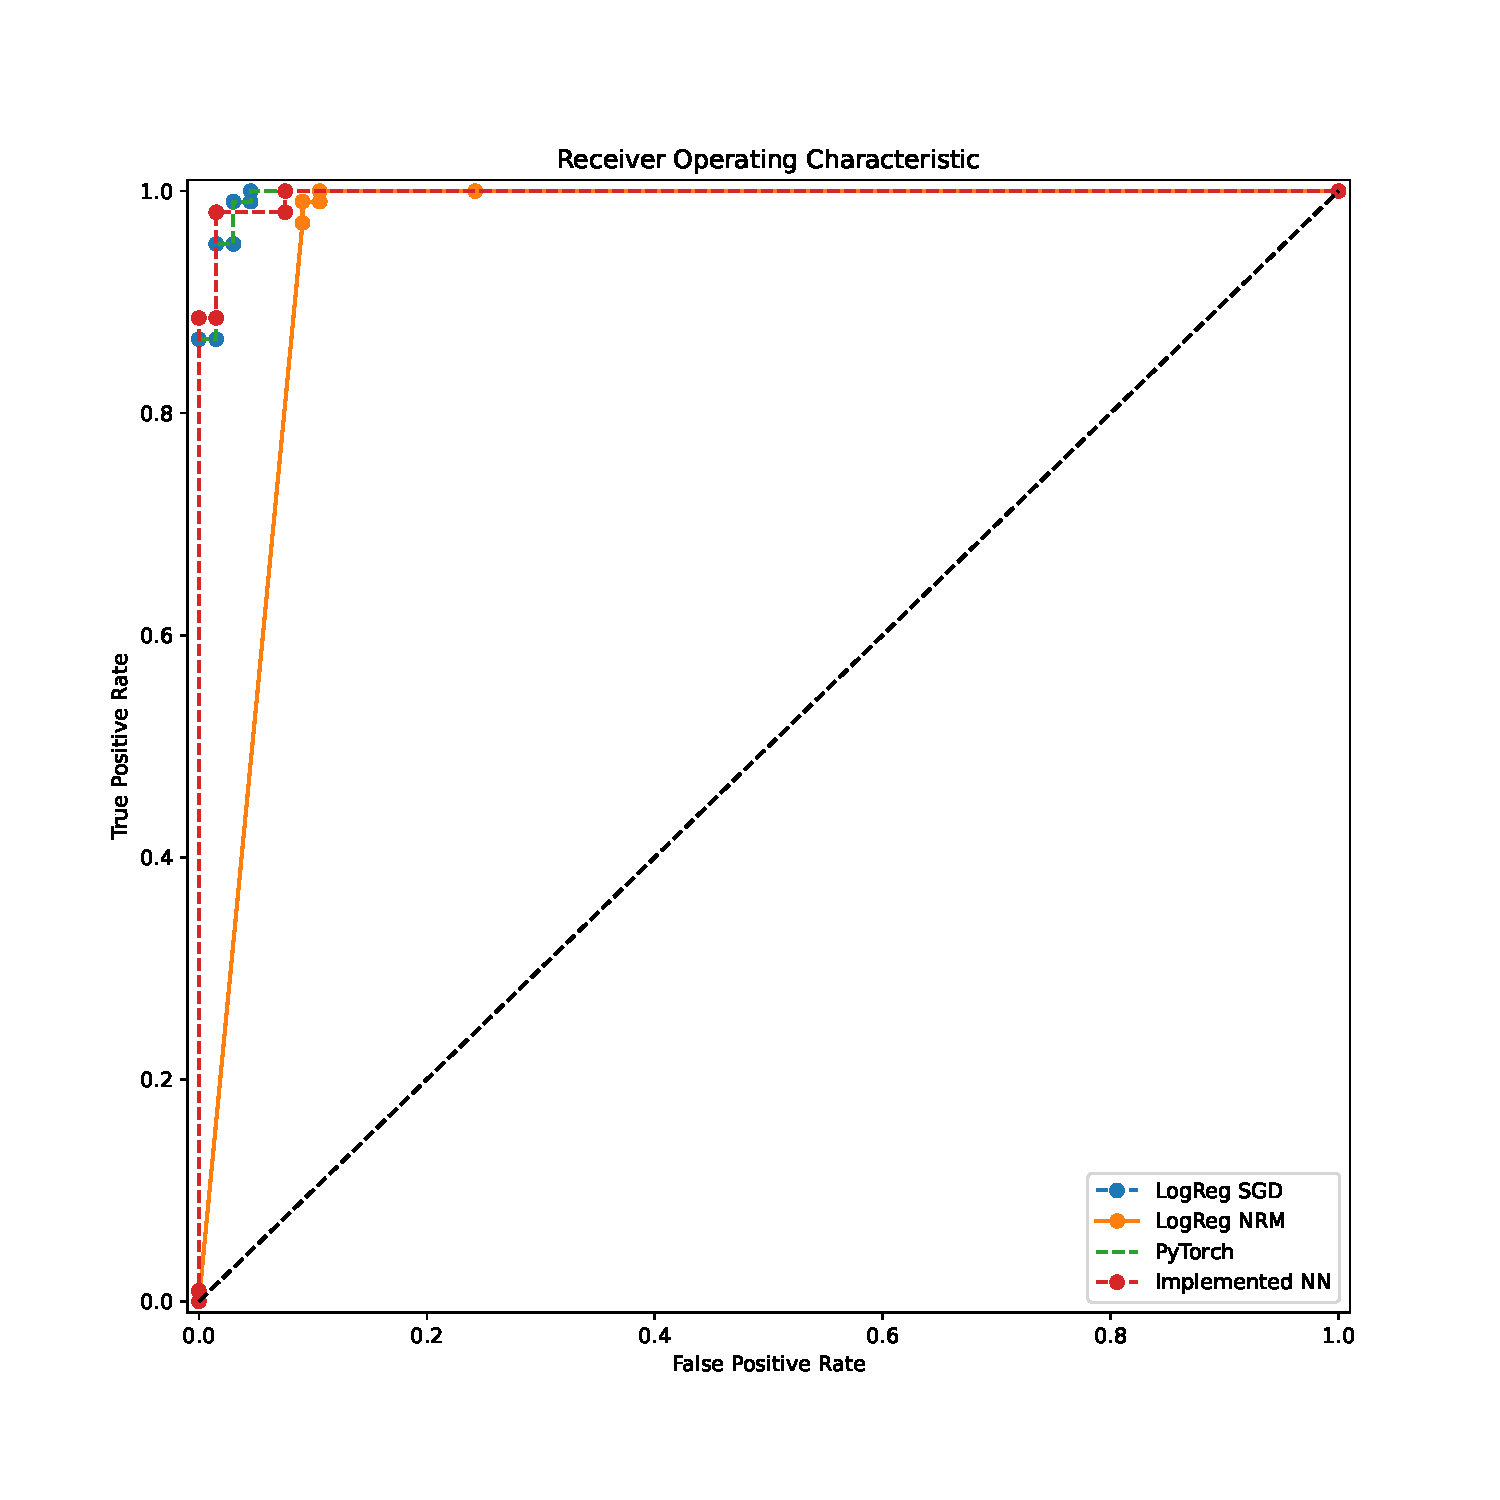
\includegraphics[width=\columnwidth]{figures/EX_E_roc_curve.pdf}
  \caption{\label{fig:EX_E_roc_curve}Comparison of ROC-curves for all classification algorithms}
\end{figure}


\section{Discussion}
\subsection{Analyzing our Stochastic Gradient Descent implementation}
As described in the introduction, all results above are generated using the Terrain data from Project 1 with the same data preprocessing and a fixed degree of 6. The degree was chosen as a compromise between complexity to the data and complexity to the computations.
Figure (\ref{fig:a_mse_epoch}) shows the epoch dependance of the SGD algorithm measured in MSE. As can be seen in the figure, as the number of epochs are increased, the MSE is reduced. In this specific case, the reduction of MSE tend to closely follow a parabola, though for 100 epochs the MSE is reduced somewhat more than average. As such, the MSE seem to converge somewhere around 0.48, which is the approximate value at 300 epochs. However, though it can clearly be seen that a higher amount of epochs results in a more precise estimation of the predictors, the computational time for each run increases with epochs as seen in Table (\ref{tab:a_epoch_run}). Hence, as a consequence of running some of the computations on an Intel(R) Core(TM) i5-3230M CPU @ 2.60GHz, the number of epochs are constrained to 100 for further computations. Though we acknowledge that 100 epochs are not necessarily the optimal number of epochs if just concerning the MSE.

Inspecting Figure (\ref{fig:a_bs}), it can be clearly seen that the lowest MSE values are attained for a batch size around 3 to 6 samples per batch. For batch sizes 8 and larger, the MSE tend to continuously increase following a weak slope. On the other hand, reducing the batch size to 2 samples per batch severely increases the MSE. Furthermore, for a batch size of 1 sample per batch, the MSE is not returned to due computational overflow (not shown). By combining the results of Figure (\ref{fig:a_mse_epoch}) and (\ref{fig:a_bs}), we can conclude that Stochastic Gradient Descent on the Terrain data performs optimal if given a descent number of epochs and a batch size of approximately 4. However, as previously discussed concerning computational resources, we have considered 100 epochs with a batch size of 4 the optimal when generating the Stochastic Gradient Descent results.

The two heatmaps shown in Figures (\ref{fig:a_gs}) and (\ref{fig:a_gslr}) show the effect of the learning rate $\eta$ as well as the l2 regularization term $\lambda$ without and with a learning rate scheduler respectively. By comparing the two plots, it can be seen that the learning rate scheduler causes all but one model to attain higher MSE. Which might be a result of too aggressive scheduling.

Moreover, a secondary observation of the inclusion of the learning rate can be pointed out. By comparing the two rightmost columns of Figure (\ref{fig:a_gs}) and (\ref{fig:a_gslr}), it can be seen that SGD differ greatly in MSE value for $\eta=0.00001$ regardless of regularization parameter. This might be an effect of scheduling the learning rate, in combination with the learning rate being initialized to such a low value that the model is unable converge in time of the scheduling reducing all movement along the gradient. Furthermore, the difference in MSE between the model for higher learning rates is not as great as for $\eta = 0.00001$, which then might be a result of the model reaching close to a minima before scheduling.

Figure (\ref{fig:a_gs}) shows that the optimal hyperparameters for our SGD algorithm given the current dataset, is $\eta = 0.01$ and $\lambda = 0.0001$. As such, Figure (\ref{fig:a_gs}) suggests that less regularization leads to lower attained MSE. This complies with the results of Table (\ref{tab:a_mse}), were an even lower MSE value is attained when noe regularization is present. Furthermore, by comparing the Ridge regression value in Table (\ref{tab:a_mse}) with the OLS value, it can be seen that OLS scores better than Ridge regression for the optimal regularization parameter as found in Figure (\ref{fig:a_gs}). These results are in line with what we discovered in Project 1 when analyzing our Ridge Regression algorithm and OLS algorithm on the same Terrain data, namely that OLS scores better in regards to MSE than Ridge.

By comparing the values in Table (\ref{tab:a_mse}), it can be seen that
the MSE values computed with our SGD algorithm gets close to the Ridge regression value, with an approximate difference of 0.1 for SGD without learning rate scheduler. Moreover, our SGD outperforms that of SciKit-learn, which is more than doubled of our computed MSE values. The same trends can be seen for the OLS case in Table (\ref{tab:a_mse}). Our SGD algorithm outperforms that of SciKit-learn also when no regularization is present.

Another note when discussing Table (\ref{tab:a_mse}) is the inclusion of Momentum SGD as described in Algorithm (\ref{alg:msgd}). With the added momentum parameter, lower MSE values are attained as all the hyperparameters are kept the same. Though the values are not as good as normal SGD without the learning rate scheduler. This could be a result of Momentum SGD requiring a learning rate scheduler to be able to run without overflow, with the same reasoning as when discussing Figure (\ref{fig:a_gs}) and (\ref{fig:a_gslr}).

\subsection{Arificial Neural Net - Regression problem}
To quantify the power of our neural network model, we studied how well the network performed relative to results obtained using Ordinary Least Squares (OLS) in project 1. Our best fit for the OLS model was MSE equal to 0.1601 as shown in figure \ref{??}, which served as our initial reference score for the NN model. For the models to compete on similar terms, we reused the same image patch from project 1 and fitted our NN on the same data using the same scaling process. We scale both the x and y input coordinates and the targets by subtracting their respective mean values. For the OLS fit, we feed the model using degree 10 for both the x and y coordinates for the OLS fit, which seeded the model with 65 features to work on. One significant difference for our Neural Net is that we only feed the NN model with the raw data, meaning we input the first-order inputs of x and y, two features in total. By doing this, the NN model receives the task of finding the optimal polynomial and its degree, and this will be incorporated within the different layers and neurons of its Neural Net. For a well-implemented Neural Net, it is often beneficial to leave it to the model to find the optimal relationships rather than seeding it to look for a specific degree. To be fair, the true optimal degree is unknown even though we approximated the best fit to be of degree 10 for the OLS model specifically. Seeding the NN to match a specific degree as done for the OLS can go both ways; it can help the NN model converge faster with a better fit, but it can also restrain the model with too little or too much unnecessary input data. Feeding the NN model with too many features can also result in the model reaching the curse of dimensionality issue at some point, leaving the model with a worse fit, since having too many features may result in an increased level of noise. A common way to tackle too many features is to use the Principal Component Analysis (PCA) algorithm. This will extract the most essential features. However, increasing the number of degrees in our design matrix (order of magnitude of our raw input) and applying PCA on it is not a good choice in this case. Such an approach yields dependent input data when the higher level feature are constructed from the order of magnitude of the raw data; thus, the condition for using PCA is not met. This left us with the most optimal approach for input feature for the Neural Net to just being the coordinates x and y from the input data. One of the major challenges of training a network full of neurons is the choice of hyper parameter. A common way to find good hyperparameters is to traverse parts of the parameter space by using a grid search.

\subsubsection{Optimal parameters}
For finding optimal hyperparameters we utilized a grid search for different hyperparameters as shown in table \ref{??}. We decided to keep batch size and number of epochs constant to limit our options for computational reasons.  We ran grid search with the chosen hyperparameters for all three activation functions; Sigmoid, RELU, and Leaky RELU, using both the small and the large network architecture shown in figure \ref{xx}.  The most optimal MSE values from the grid search can be found in the heatmaps for all the three activation types; Sigmoid in figure \ref{FIG5 a}, RELU in figure \ref{FIG6 a}, Leaky RELU in figure \ref{FIG7 a}. Figure \ref{FIG5 b}, \ref{FIG6 b}, and \ref{FIG7 b} shows how the similar Tensorflow model performs on the same grid search parameters. The most optimal hyperparameters for each activation function is summaries in table \ref{x}, \ref{x}, and \ref{x}.


\subsubsection{Parameters and model complexity}
Figure \ref{fig:NN_model_complexity} is showing how the model performance is connected to complexity. The plot is showing MSE performance for all the six model complexities having $33,65,129,325,1211,4629$ parameters relative to the hyperparameters used during grid search. The small model architecture consisting of only one hidden layer is relating to parameter sizes $33,65,129$. The large model architecture consisting of three hidden layers where the second hidden has twice the debth (neurons) as the first and last layer, and the large architecture is relating to parameter sizes $325,1211,4629$. The vertical line in the plot for each parametercount is not a standard deviation, but it shows how the MSE varies relative to the different hyperparameters used during grid search. A complete grid search was conducted for all the six parametercounts. The variation in MSE performance for each parametercount indicates how sensitive the model is to the hyperparameters considering the activation function and the model complxity.\\\\

\textbf{The sigmoid activation function}\\
The sigmoid function seems to be the activation function more sensitive to hyperparameters out of all the activation functions tested, and the vertical lines in figure \ref{fig:NN_model_complexity} for the sigmoid function looks to superseed the others in variation. Moreover, the sigmoid function seems to fit slightly better for small architectures having smaller complexity and fewer parameters. It looks like the sigmoid function is not able to harness the potential of increased model complexity that well. The sigmoid function is know to saturate at the upper and lower bounds, and this may lead to the gradients being washed out during training. This can in turn lead to the known vanishing gradient problem. Looking at the plot, we believe that the known problems with the sigmoid activation is surfacing within the figure, and that it is clear that the sigmoid is not being as potent as RELU and Leaky RELU in terms of performance and robustnes to hyperparameters.\\\\

\textbf{The RELU activation function}\\
The RELU activation function seems to tackle higher model complexity comparing the sigmoid activation function as shown in figure \ref{fig:NN_model_complexity}. The MSE values using RELU are decreasing as the model complexity is increasing considering MSE relative to all hyperparameters indicated in the vertical line. The vertical lines for RELU spans a relatively short range of MSE values especially for lower model complexity, and this indicates that the RELU is maximizing the potential in smaller model complexities better than sigmoid regardless of the choice of hyperparameters. Comparing sigmoid with the RELU, it seems that RELU is able to harness the potential residing within increased model complexity better. The lowest MSE values are achieved at the highest tested model complexity using the large architecture having 4629 parameters. The reason for this improvement looks to be that the RELU do not saturate the same way as the sigmoid function. We also discovered that the RELU greatly benefits from the He initializations of weights \cite{He2015} in terms of model performance. The positive effect initializing the weights using the HE approach versus plain normal distribution is significant. Before we introduced the HE initialization the RELU model performed similar to the model using sigmoid activation. Using the RELU activation function our model often encountered float64 overflow, cause of gradient explosion, and our model was very sensitive high learning rate and high lambda values for regularization. Applying the HE weight initialization drastically improved overflow issue and made our model more robust to hyperparameters. We were able to push learning rate as high as 0.1 with the HE initialization, and than discovered our best fit using a learning rate of 0.1. Furthermore, given the trend that MSE gets better at higher learning rates and higher model complexity as seen in figure \ref{fig:NN_model_complexity} we believe that there is even greater potentials than what we had time to discover for our model when using RELU and HE initialization.\\\\

\textbf{The Leaky RELU activation function}\\
Building on the results and experiences using the RELU activation function, we ventured into the domain of the Leaky RELU activation function. As shown in \ref{fig:NN_model_complexity} the results from the Leaky RELU activation function is further improving model performance over RELU for some hyperparameter combinations. It looks that Leaky RELU is more sensitive to the usage of hyperparameters given the longer vertical lines for Leaky RELU over its RELU sibling. However, it looks that the Leaky RELU have slightly more potential in terms of pure MSE minimization for some combination of hyperparameters over RELU.

\subsubsection{Performance of activation functions}
Comparing the best results for the different activation functions in table \ref{tab:grid_search_optimal_sigmoid}, \ref{tab:grid_search_optimal_RELU},\ref{tab:grid_search_optimal_Leaky_RELU}, the Sigmoid function has the highest MSE value. RELU is performing significantly better than Sigmoid, and the best performing activation function is the Leaky RELU.

\subsubsection{Effect of weight initialization}
We first tried to initialize the weights only using gaussian distribution with $\sim N(0,1)$ for all activation functions. When implementing the HE \cite{He2015} method for RELU and Leaky RELU, and Xavier \cite{Glorot2010} for Sigmoid we immediately got significantly better performance than with our initial weight initialization. When using the more optimal weight initialization strategies we also discovered less problems of exploding gradients during in the model training especially for RELU and Leaky RELU.


\subsubsection{Own Neural Net vs Tensorflow}
Figure \ref{fig:own_NN_vs_tf} shows how our best performing NN model architecture compares to a similar architecture implemented in Keras (Tensorflow). The figure shows a plot of the MSE values from the grid search using several combinations of hyperparameters. The x-axis represents a fitted model using one specific hyperparameter combination. The hyperparameters combination is equal for our own NN and the tensorflow model. The y-axis is MSE between test set true target and predicted for the given model on the x-axis.


\subsubsection{Neural Net vs Ordinary Least Squares on terrain data}
Comparing our best fitted NN with the best OLS fit in project 1 is shown in figure1. It is clearly that our NN outperforms the OLS model in terms of MSE.

In figure \ref{x} and \ref{y} we see that the NN model is more greedy than the OLS model when it comes to minimizing errors. It looks like the NN model prioretizing parts in the terran
where it is more beneficial to minimize the error. E.g., minimizing along the deep valey and along the cliff. These are parts of the terrain that potentials yields the large error due to the steep
variation in the terrain. Albeit Figure (\ref{fig:2D_preds_NN_vs_OLS}, c) fits the finer details in the original terrain to a larger extent than (\ref{fig:2D_preds_NN_vs_OLS}, b), this is circumvented by its inability to precisely fit these details. Thus yielding a positive gain to the MSE. As such, it might seem more productive to precisely fit some structures while disregarding other structures when fitting the terrain data, with regards to lowering the MSE.

This might be a derived result from the Bias-Variance tradeoff which we thourgly discussed in Project 1, were we studied MSE as result of model generalizability. Moreover, we concluded that a overfitted model in terms of its own training data would have difficulties correctly fitting new data. As the Neural Net predicts a new value using a significantly smaller amount of predictors in comparison to the OLS model $(2 < 65)$, the model is not forced by the composition of predictors to fit a certain way. Which is reflected in the lack of structures in the fitted terrain compared to OLS as seen in Figures (\ref{fig:2D_preds_NN_vs_OLS}) and (\ref{fig:3D_preds_NN_vs_OLS}). However, the smaller amount of predictors does not imply that the Neural Network would not be able to overfit. Had the Neural Network been trained on fewer datapoints, the threshold for overfitting the model could have been reached at an earlier epoch.


\subsubsection{Robustness of our Neural Net}
In the same manner as in Project 1, we implemented the k-fold Cross Validation resampling technique to study the robustness of the reported MSE values. Note that due to model overflow using the optimal architecture setup, we used $\eta = 0.05$ instead of $\eta = 0.1$ with large architecture. As seen in Table (\ref{tab:cross_val_scores}), there is a steady overall performance except for fold 5. This might be a consequence of the nature of the terrain data resampling, were fold 5 contains more complex terrain compared to other folds. Moreover, the less optimal results might be a consequence of the suboptimal model configuration.

\subsection{Classification using our Neural Network}
As stated in the Results, we followed the process outlined in the Methods section when we made our Neural Network compliant with classification problems. As a note, the rest of the Neural Network architecture and internal methods are the same for regression and classification. The initial architecture was chosen to be similar to the large architecture in Figure (\ref{fig:large_architecture}), with 32 nodes in the first hidden layer which is then doubled in the second hidden layer then halved back to 32 in the last hidden layer. The dimension of the output layer is governed by the nature of the target data. In this case, we only work on binary classification problem, which translates to a single output in contrast to a multiclass problem. For the latter, the size of the output layer would be dictated by the number of classes, with target data being one-hot encoded.

With the initial architecture, we ran two separate grid searches for both our own Neural Network as well as the one implemented using PyTorch. For our own Neural Network, the grid search returned $\eta=0.1$ and $\lambda = 0.0$ as optimal parameters with an Accuracy score (\ref{eq:acc}) of $0.9824$, whereas PyTorch got $\eta = 0.002$, $\lambda = 0.00001$ and the same Accuracy score. Figure (\ref{fig:conf_matrix_home_torch}) plots the associated confusion matrices for the just described models. Figure (\ref{fig:conf_matrix_home_torch}) demonstrates how two classification models can attain the same Accuracy score, albeit their predictions are distributed differently. Our Neural Network has an additional false negative not seen in the PyTorch network, although the PyTorch model has an additional False positive such that the total sum of misclassifications is equal. This is also reflected in their correct classifications as a direct consequence of their misclassifications.

\subsubsection{Complexity of Stochastic Gradient Descent and Newton Raphson for Logistic Regression}
When implementing the Logistic Regression method, we followed both Algorithm (\ref{alg:lsgd}) and (\ref{alg:newtonraphson}) as they result in two different approaches to gradient optimization.
As demonstrated by Algorithm (\ref{alg:lsgd}) and (\ref{alg:newtonraphson}), there are several distinct differences between the two implementations. While Newton Raphson´s method only iterates through the epochs, the stochastic gradient descent will have additional iterations through the batches. This might lead to the impression that the latter is computationally more complex than the first. This is however not the case, as the inversion of a $k \times k$ matrix has a complexity of $O(k^3)$, which has to be carried out for each iteration as the parameters change with every update \cite{Goodfellow2016}. For cases with a large number of parameters, the exponentially increasing computational burden imposed often makes SGD the preferred solver. % SGD being the poor man's choice - Morten

\subsubsection{Comparing the Neural Network with Logistic Regression}
Compared to Stochastic Gradient Descent which has approximated the Hessian with the learning rate $\eta$, Newton Raphson iteratively computes the first and second derivative for each epoch. As such, it would not be possible to do a similar grid search for both models, as they require different hyperparameter. Thus, we only do a grid search for Logistic Regression with Stochastic Gradient Descent which can be seen in Figure (\ref{fig:EX_E_logreg_gridsearch}). By inspecting Figure (\ref{fig:EX_E_logreg_gridsearch}), it can be seen that a model with a high learning rate $\eta = 0.1$ and l2 regularization term approaching 0. Though it is difficult to assert which hyperparameters are optimal, as the optimal region in Figure (\ref{fig:EX_E_logreg_gridsearch}) contains many viable combinations. Though there seems to be a clear trend towards a model with higher learning rate and less l2 regularization within the parameter space.

Using the hyperparameters obtained from the SGD Logistic Regression grid search in Figure (\ref{fig:EX_E_logreg_gridsearch}), the confusion matrices for both Logistic Regression methods are shown in Figure (\ref{fig:conf_matrix_sgd_nrm}). By inspecting Figure (\ref{fig:conf_matrix_sgd_nrm}), it can be seen that the results agree less than when inspecting Figure (\ref{fig:conf_matrix_home_torch}). The difference in accuracy become evident when looking at the number of both false positives and negativess. We note that there is no regularization term added to the Newton Raphson equation, which could have resolved some misclassifications if the Hessian matrix was e.g. non positive definite. Moreover, the Stochastic Gradient Descent approach does not lead to any false negatives. This might be a result of limited data, were no data points match the criterion for the model to misclassify accordingly.

Finally, Figure (\ref{fig:EX_E_roc_curve}) summarizes all implemented models in a Receiver Operating Characteristic plot. Figure (\ref{fig:EX_E_roc_curve}) demonstrates the performance of all four classification models without regards to some pre-set threshold. The optimal area under the curve for a ROC-plot equals $1$, which translates to the model being able to perfectly distinguish all positives and negatives correctly. As can be seen, all our models achieves an area under the roc-curve $\approx 1$, which follows what we already have seen in the confusion matrices for the case of a threshold $ = 0.5$. It is difficult to determine which model performs best, though it can be clearly seen that Newton Raphson performs considerably worse with a higher false positive rate as also seen in Figure (\ref{fig:conf_matrix_sgd_nrm}).

\section{Conclusions}
Throughout this Project, we have studied the behaviour of our own implementation of a Feed Forward Neural Network with regards to both the fitting of a terrain as well as classification of breast cancer. We started by implementing Stochastic Gradient Descent, which we used as a reference when developing other Gradient optimizer-methods such as Logistic Regression and the aforementioned Neural Network. All our own implementations were also benchmarked against their similar counterparts using SciKit-learn, TensorFlow and PyTorch.

When studying the Stochastic Gradient Descent, we saw that the learning rate scheduler which we implemented severely prohibited the gradient from moving, especially for low initial learning rates. Moreover, we found that when applied to the terrain data, it performed optimally when $\eta = 0.01$ and no l2 regularization. With this setup, our SGD was able to reach MSE values of $0.4172$ which is slightly larger than the OLS counterpart of $0.3216$ at the same degree 6. As such, we gain no confidence in using our SGD algorithm as a replacement for the OLS from Project 1, relative degree 6. Though other degrees have not been thoroughly explored, we consider it reasonable to assume that SGD would not outperform OLS even at other degrees.

Moving on to Neural Networks for regression, the architecture in combination with hyperparameters resulted in several models which were able to outperform our benchmark OLS from Project 1. This served as motivation when further tuning the hyperparameters for finding the model fit using grid search, which the result can be seen in both Figure (\ref{fig:2D_preds_NN_vs_OLS}) and (\ref{fig:3D_preds_NN_vs_OLS}). The most critical factor for model performance when fitting the terrain data seemed to be the activation function together with weight initialization. As expected, the sigmoid function was out performed by the ReLU function which itself was superseded by the Leaky ReLU. Though as alluded, the ReLU function family required He initialization instead of a normal distribution of the weights to be able to reach the reported results. Moreover, $\eta = 0.1$, no l2 regularization together with a Leaky ReLU, HE weight initialization and a large model architecture containing 4629 individual parameters defined our optimal Neural Net configuration. With this architecture, the model was able to achieve an MSE of $0.0971$ in the predicted terrain fit compared to OLS from Project 1 which scored an MSE of $0.1602$, as seen in Figures (\ref{fig:2D_preds_NN_vs_OLS}) and (\ref{fig:3D_preds_NN_vs_OLS}). Thus our Neural Network is able to outperform the OLS from Project 1 with respect to degree $10$ (65 predictors), which also was found to be the optimal fit of OLS.

In studying the Wisconsin Breast Cancer Data, we saw that all models performed well above a accuracy of $0.9$. Though the preferred model is tied to the classification problem in question, for our dataset all models performed relatively equally except for Newton Raphson which posed a higher misclassification rate. However, not all models are computationally equal, and with regards to computational efficiency as well as a high Accuracy, one could make an argument for Logistic Regression with Stochastic Gradient Descent beeing the preferred model. However, behind the the high obtained accuracy, one can see from figure (\ref{fig:conf_matrix_sgd_nrm}) that the Stochastic Gradient Descent produced 4 false positives. In the context of breast cancer screening, this would be a highly undeseriable behaviour, as this would result in 4 samples beeing predicted as non-cancerous tumour, when the reality is the opposite.  However, this result might also simply arise from the limited size and complexity of the dataset, as it would not seem reasonable for our model to never misclassify a positive.

While working on this Project, we have seen that a Neural Network is able to outperform regression methods given the right architecture. However, though we have tried to explore different hyperparamter combinations through extensive use of grid search, we note that our final model could be outperformed given other unexplored hyperparameter combinations. Furthermore, our Neural Network is implemented in such a way that extending the model with new activation functions, cost functions, weight initializations, gradient clipping and more is relatively simple. Though we have limited itself to three activation functions, two different weight initializations and Stochastic Gradient Descent, improving upon these methods would probably achieve even better results.

Finally, this project have demonstrated the power of the Universal approximation Theorem. We have seen that Neural Networks aptly fit complicated data, even with sparse input dimensionality. Though Regression methods do have their use, especially with regards to computational efficiency and simplicity. With increasingly complex data, is is difficult to disregard the adaptability and extendability made possible with Neural Networks.

\appendix

\section{Source Code}
\label{sec:sc}
Link to github repository containing all developed code for this project: \url{https://github.com/AndreasBordvik/FYS-STK4155-Prj2_report}

\section{Additional Figures}
For a directory containing additional Figures and models, we refer to to the Appendix located in our GitHub: \textbf{LINK TO APPENDIX}

% Create the reference section using BibTeX:

% ------------------- end of main content ---------------

\bibliographystyle{plain}
\bibliography{biblio}




\end{document}